% !TeX program = xelatex
% !TeX encoding = UTF-8
% 正文内容源：BEST_重构初稿_v16.docx；双栏模板按中文稿件模板（202608更新）配置。
\documentclass{dcfp}
\usepackage{array}
\usepackage{ragged2e}
\usepackage{flushend}
\usepackage{cuted}
\usepackage{placeins}
\usepackage{textcomp}
\usepackage{url}
\usepackage{needspace}
\usepackage{longtable}
\def\UrlBreaks{\do\/\do-\do\_\allowbreak{}}
\frenchspacing
\xeCJKsetup{CJKglue={\hskip 0pt plus 0.06em minus 0.02em},CJKecglue={\hskip 0.15em plus 0.04em minus 0.03em}}
\definecolor{phbg}{RGB}{255,244,130}
\newcommand{\PH}[1]{\begingroup\setlength{\fboxsep}{0.4pt}\colorbox{phbg}{\strut #1}\endgroup}
\newcommand{\tabnote}[1]{\par\vspace{2bp}{\fontsize{9bp}{13bp}\selectfont\noindent #1\par}\vspace{2bp}}
\renewcommand{\CNTitle}[1]{\par\vspace{2bp}{\centering\heiti\fontsize{14bp}{18bp}\selectfont #1\par}}
\renewcommand{\CNAuthors}[1]{\par\vspace{2bp}{\centering\kaishu\fontsize{10.5bp}{15.6bp}\selectfont #1\par}\vspace{2bp}}
\renewcommand{\CNAffiliation}[1]{{\centering\songti\fontsize{9bp}{14.5bp}\selectfont #1\par}}
\renewcommand{\CNAbstract}[1]{\par\vspace{3bp}{\kaishu\fontsize{9bp}{12.5bp}\selectfont\noindent{\heiti 摘\quad 要：}#1\par}}
\renewcommand{\CNKeywords}[1]{\par\vspace{2bp}{\kaishu\fontsize{9bp}{13.5bp}\selectfont\noindent{\heiti 关键词：}#1\par}}
\renewcommand{\ENTitle}[1]{\par\vspace{3bp}{\centering\bfseries\fontsize{14bp}{17bp}\selectfont #1\par}\vspace{1bp}}
\renewcommand{\ENAuthors}[1]{\par\vspace{1bp}{\centering\fontsize{10.5bp}{14.5bp}\selectfont #1\par}\vspace{1bp}}
\renewcommand{\ENAbstract}[1]{\par\vspace{1bp}{\fontsize{9bp}{9.3bp}\selectfont\noindent\textbf{Abstract: }#1\par}\vspace{1bp}}
\renewcommand{\ENKeywords}[1]{{\fontsize{9bp}{10bp}\selectfont\noindent\textbf{Keywords: }#1\par}\vspace{1bp}}
\ctexset{section={format=\heiti\fontsize{10.5bp}{15.6bp}\selectfont}}
\titlespacing*{\section}{0pt}{6bp}{3bp}
\titlespacing*{\subsection}{0pt}{4bp}{2bp}
\titlespacing*{\subsubsection}{0pt}{3bp}{2bp}
\setlength{\textfloatsep}{7bp plus 1bp minus 1bp}
\setlength{\floatsep}{7bp plus 1bp minus 1bp}
\setlength{\intextsep}{6bp plus 1bp minus 1bp}
\setlength{\abovedisplayskip}{5bp plus 1bp minus 1bp}
\setlength{\belowdisplayskip}{5bp plus 1bp minus 1bp}
\setlength{\abovedisplayshortskip}{3bp}
\setlength{\belowdisplayshortskip}{4bp}
\renewcommand{\topfraction}{0.92}
\renewcommand{\bottomfraction}{0.85}
\renewcommand{\textfraction}{0.06}
\renewcommand{\floatpagefraction}{0.78}
\setcounter{topnumber}{3}
\setcounter{bottomnumber}{2}
\setcounter{totalnumber}{5}
\makeatletter
\setlength{\@fptop}{0pt}
\setlength{\@fpsep}{7bp}
\setlength{\@fpbot}{0pt plus 1fil}
\makeatother
\emergencystretch=1.4em
\widowpenalty=10000
\clubpenalty=10000
\displaywidowpenalty=10000
\captionsetup{justification=raggedright,singlelinecheck=false,skip=3bp}
\setlength{\tabcolsep}{2pt}
\renewcommand{\arraystretch}{1.08}
\funding{}
\correspondence{\PH{作者名（E-mail：待补充）}}
\begin{document}
\FirstPageNotes
\CNTitle{\textbf{面向天文档案的科学语义约束智能体数据访问方法\\——BEST 实现与评价}}
\CNAuthors{\PH{作者姓名}\PH{¹}\PH{，通信作者}\PH{¹,*}}
\CNAffiliation{\PH{¹ }\PH{单位名称，部门，城市}\PH{ }\PH{邮编；}\PH{*}\PH{通信作者}\PH{ E-mail}\PH{：待补充}}
\CNAbstract{【目的】研究如何将自然语言科学需求转化为可执行、状态可辨且证据可追溯的数据访问，并使科学陈述遵守数据的语义与适用边界，以 BEST（BEst STar）测光标准星数据库为实现与验证对象。【方法】区分面向模型决策的指导信息与面向查询过程的执行机制：前者提供字段语义、单位约定、能力边界和证据使用要求；后者实施参数校验、查询状态管理、分页与截断检查及结果结构核验。通过输入契约和统一结果结构连接两层，并实现表访问协议（Table Access Protocol，TAP）与天文数据查询语言（Astronomical Data Query Language，ADQL）网关。使用 deepseek-v4.1-flash 模型，分别评价操作正确性、科学语义忠实度和运行一致性。【结果】工具映射加权分均值为 0.9530；21 个固定查询场景的三次重复均通过，15 个协议故障场景均按约定处置。完整配置的关键科学断言命中率为 90.14\%，较基础包装器高 23.94 个百分点，反映完整机制与领域材料的组合效果。相同原子工具条件下，完整指导配置的规则通过率为 56.55\%，较原子工具基线高 7.14 个百分点，平均工具调用与输出 token 分别减少 32.95\% 和 12.44\%。固定回包及有效记录条件下，工具序列与核心结论一致性分别为 0.8637 和 0.8673。【结论】分层设计使模型的数据理解与程序的契约执行能够分别评价并相互衔接。BEST 实验支持所测场景的契约符合性及指导信息的任务表现，为其他天文档案提供设计参考。}

\CNKeywords{天文数据库；大语言模型智能体；智能体数据访问；数据来源追溯；科学语义忠实度}
\ENTitle{\textbf{Agent Data Access to Astronomical Archives under Scientific Semantic Constraints: Implementation and Evaluation with BEST}}
\ENAuthors{\PH{【}\PH{NAME Namename}\PH{】}1, \PH{【}\PH{NAME Namename}\PH{】}1*}
\ENAffiliation{1．\PH{【}\PH{Department of ****, University, City Zip code, China}\PH{】}}
\ENAbstract{[Objective] This study investigates how agents can translate natural-language scientific requests into executable, state-aware and traceable data access while respecting the semantics and applicability of the data, using the BEst STar (BEST) database for implementation and evaluation. [Methods] The design separates model-facing guidance from query-execution mechanisms. Guidance specifies field semantics, units, capability boundaries and evidence-use requirements; execution mechanisms validate parameters, manage query states, check pagination and truncation, and verify result structures. Input contracts and a unified result structure connect the two layers. A Table Access Protocol (TAP)/Astronomical Data Query Language (ADQL) gateway supports standard clients. Experiments with deepseek-v4.1-flash separately evaluate operational correctness, scientific-semantic faithfulness and repeated-run consistency. [Results] The mean weighted tool-mapping score was 0.9530. All three repetitions of 21 fixed-query scenarios passed, and all 15 protocol-fault scenarios were handled as specified. The full configuration achieved 90.14\% critical-assertion recall, 23.94 percentage points above the baseline wrapper, reflecting the combined effect of access mechanisms and domain materials. With the same atomic tools, full guidance achieved a 56.55\% rule-based pass rate, 7.14 percentage points above the atomic-tool baseline, with 32.95\% fewer tool calls and 12.44\% fewer output tokens. Under fixed-response replay and valid-record conditions, tool-sequence and core-conclusion consistency were 0.8637 and 0.8673. [Conclusions] The layered design enables separate evaluation and coordinated use of model-level data understanding and programmatic contract enforcement. The BEST experiments provide evidence for contract conformity in the tested scenarios and for guidance-informed task performance, offering design references for other astronomical archives.}

\ENKeywords{astronomical database; large language model agent; agent data access; data provenance; scientific-semantic faithfulness}



\begin{PaperBody}
\section*{引言}

在 BEST 归档测光数据的智能体访问中，自然语言请求往往省略星表口径、坐标单位或查询范围，字段名称也不足以表达测光来源与适用条件。若模型直接将其转为接口调用，可能得到格式正确但科学含义不符的结果；分页截断、空结果与查询失败相混淆还会影响数据完整性，分散的参数、状态与来源记录也增加了核对与复用难度。本文关注的核心问题是：如何使智能体将自然语言科学需求转化为可执行、状态可辨且证据可追溯的数据访问，并使最终科学陈述遵守数据的语义与适用边界？

天文巡天与归档项目持续积累多波段测光数据，星表数据的高效访问与正确解释是目标筛选与交叉匹配的基础。大语言模型驱动的智能体为自然语言科学需求与数据服务提供了新的交互方式，已有研究探索了其对瞬变源分类结果的文本解释\citep{ref1}、在端到端天文观测流程中的应用\citep{ref2}与对实验任务自动化的支持\citep{ref3}。

BEST（BEst STar）是面向测光标准星的归档数据资源，其访问入口为 \url{https://nadc.china-vo.org/data/best/}。其数据库记录与配套论文介绍了覆盖全天、200 余个通带的测光标准星数据集\citep{ref4,ref5}。访问这类数据需明确星表、字段、单位及缺失值占位符（sentinel value，即编码缺失测量的取值）的含义。BEST 原站的网页查询分两阶段：先提交查询条件取得结果集标识，再据此读取命中总数与分页记录。表访问协议（Table Access Protocol，TAP）规定表数据服务的标准接口，天文数据查询语言（Astronomical Data Query Language，ADQL）用于表达天文表查询\citep{ref6,ref13}。因此，连接标准查询入口与原站流程，还需保持参数含义、查询状态与分页完整性的对应。

工具选择研究指出，工具描述的细微变化可能影响模型在候选工具之间的选择\citep{ref7}，说明面向科学数据的工具调用需要明确的输入约束和参数语义，不能仅依赖工具名称。对于 BEST 测光档案，同一访问流程还须区分查询尚未建立、成功零行、部分返回与完整返回等状态，字段名称相似也不能替代其单位与含义的确认。因此，访问方法需将输入契约（input contract，即对请求参数结构、允许取值与必需信息的约定）与结果证据作为衔接对象。

本文研究面向天文档案的智能体数据访问方法，重点考察自然语言请求、查询执行与科学解释之间的语义衔接。针对 BEST 访问中的参数不确定与来源分散问题，本文区分面向模型的指导信息与面向查询过程的执行机制：前者提供字段语义、参数约定、能力边界与证据使用要求，辅助模型理解请求并解释结果；后者通过程序实施参数校验、查询状态管理与结果契约检查，并关联查询条件、返回记录和来源信息。两者分别作用于模型决策与查询执行，共同构成从自然语言需求到可追溯交付的访问流程。

本文的主要贡献包括：
\begin{enumerate}
\item 提出面向 BEST 的分层设计，区分指导信息与执行机制，通过输入契约与统一结果结构连接请求理解、查询执行与结果解释。
\item 实现适配 BEST 两阶段查询的访问工具与 TAP/ADQL 网关，显式区分查询失败、成功零行、部分返回与完整返回，并保留条件、数据来源与步骤关联。
\item 构建操作正确性、科学语义忠实度与运行一致性的评价方案，检验执行机制的契约符合性，以及指导信息在相同工具条件下对任务表现与开销的影响。
\end{enumerate}

\section{相关工作}

\subsection{天文数据表访问协议与科学语义}

TAP 支持同步与异步查询，ADQL 可表达空间约束等天文表查询操作\citep{ref6,ref13}。标准协议统一了客户端与数据服务之间的交互方式，但查询语法的一致一般并不自动保证字段含义、单位、缺失值约定和结果状态得到正确解释。对于 BEST 的两阶段查询流程，协议适配还需要保留查询生命周期中的状态语义。

天文数据产品的字段含义必须结合其来源文档解释。例如，Gaia 第三次数据发布（Gaia Data Release 3，Gaia DR3）的内容说明和文档为测量字段及目录标记提供了解释依据；访问时须结合具体表和字段确认其含义，不能仅凭字段名称推断观测历元数或变星属性\citep{ref8,ref9}。这一例子说明，字段名称本身不足以决定科学含义，访问过程需要保留与数据源相对应的元数据和来源信息。BEST-Skill 将这一要求落实到请求约束和结果交付中，使字段选择、执行状态、载荷及来源记录能够在同一访问流程中衔接。

\subsection{智能体工具调用与科学任务评价}

推理与行动交替方法 ReAct 将推理步骤与任务动作交替组织，使语言模型能够依据环境反馈推进任务\citep{ref10}。科学智能体评价基准 ScienceAgentBench 从数据驱动的科学发现任务出发，对智能体完成科学工作流的能力进行系统评价\citep{ref11}；科学工具智能体 SciToolAgent 则利用描述工具及其关系的知识图谱支持多工具检索与组合\citep{ref12}。相关工具选择研究还表明，候选工具的描述方式可能影响模型偏好\citep{ref7}。这些工作分别为行动组织、科学任务评价和多工具整合提供了方法基础。

与面向一般行动流程或科学工作流的评价不同，BEST-Skill 聚焦于科学档案访问链路中的参数约束、查询契约、领域语义、执行状态和结果来源。本文从指导信息和执行机制两个层次组织这些要素，并为模型任务表现、程序契约符合性和科学语义忠实度分别设置评价任务、判据与统计单位。


\section{科学语义约束下的分层访问设计}

\subsection{指导信息与执行机制}

本文以 BEST-Skill 命名面向 BEST 的具体实现，即本节所述的访问工具、TAP/ADQL 网关与统一结果信封；该实现同时作为所提出访问方法的验证对象。访问方法分为两个层次：指导信息作用于模型对请求和数据的理解，执行机制作用于具体查询操作及其结果状态；两层通过工具输入契约和统一结果结构衔接。

\begin{enumerate}
\item \textbf{指导信息：辅助模型决策。}向模型提供字段含义、单位约定、能力边界、缺失值解释和来源引用要求，并说明何时澄清、拒绝或检查结果。这些材料影响工具选择、参数组织与科学解释，其效果通过模型任务表现评价。
\item \textbf{执行机制：检查操作并记录状态。}程序实施参数校验、查询状态转换、分页与截断检查、结果结构核验以及来源和步骤记录。该层拒绝违规输入、标记不完整返回并明确记录查询结果，其契约符合性通过固定场景、故障注入和执行记录评价。
\end{enumerate}

两层可以涉及同一概念，但承担不同作用。例如，参数校验指导提醒模型补全单位，程序校验则检查已提交参数是否符合契约；结果后验证指导影响模型是否再次检查，程序结果核验则按规则检查字段、状态与记录结构。执行机制可以约束查询行为，不能据此保证模型科学解释的正确性，后者由独立的科学语义评价检验。

图~\ref{fig:architecture} 展示访问接口与执行流程的实现结构。执行层通过五状态流程和七项原子工具（星表枚举（发现可用星表）、星表描述（字段、波段与单位）、名称解析（名称转换为坐标）、坐标锥搜（检索指定天区）、批量交叉匹配（建立位置对应关系）、结果计数（读取命中总数）和分页读取（获取分页记录））完成数据访问，TAP/ADQL 网关承接标准查询；结果信封将获得的数据与执行状态、来源及处理步骤关联。

\begin{figure*}[!t]
\centering
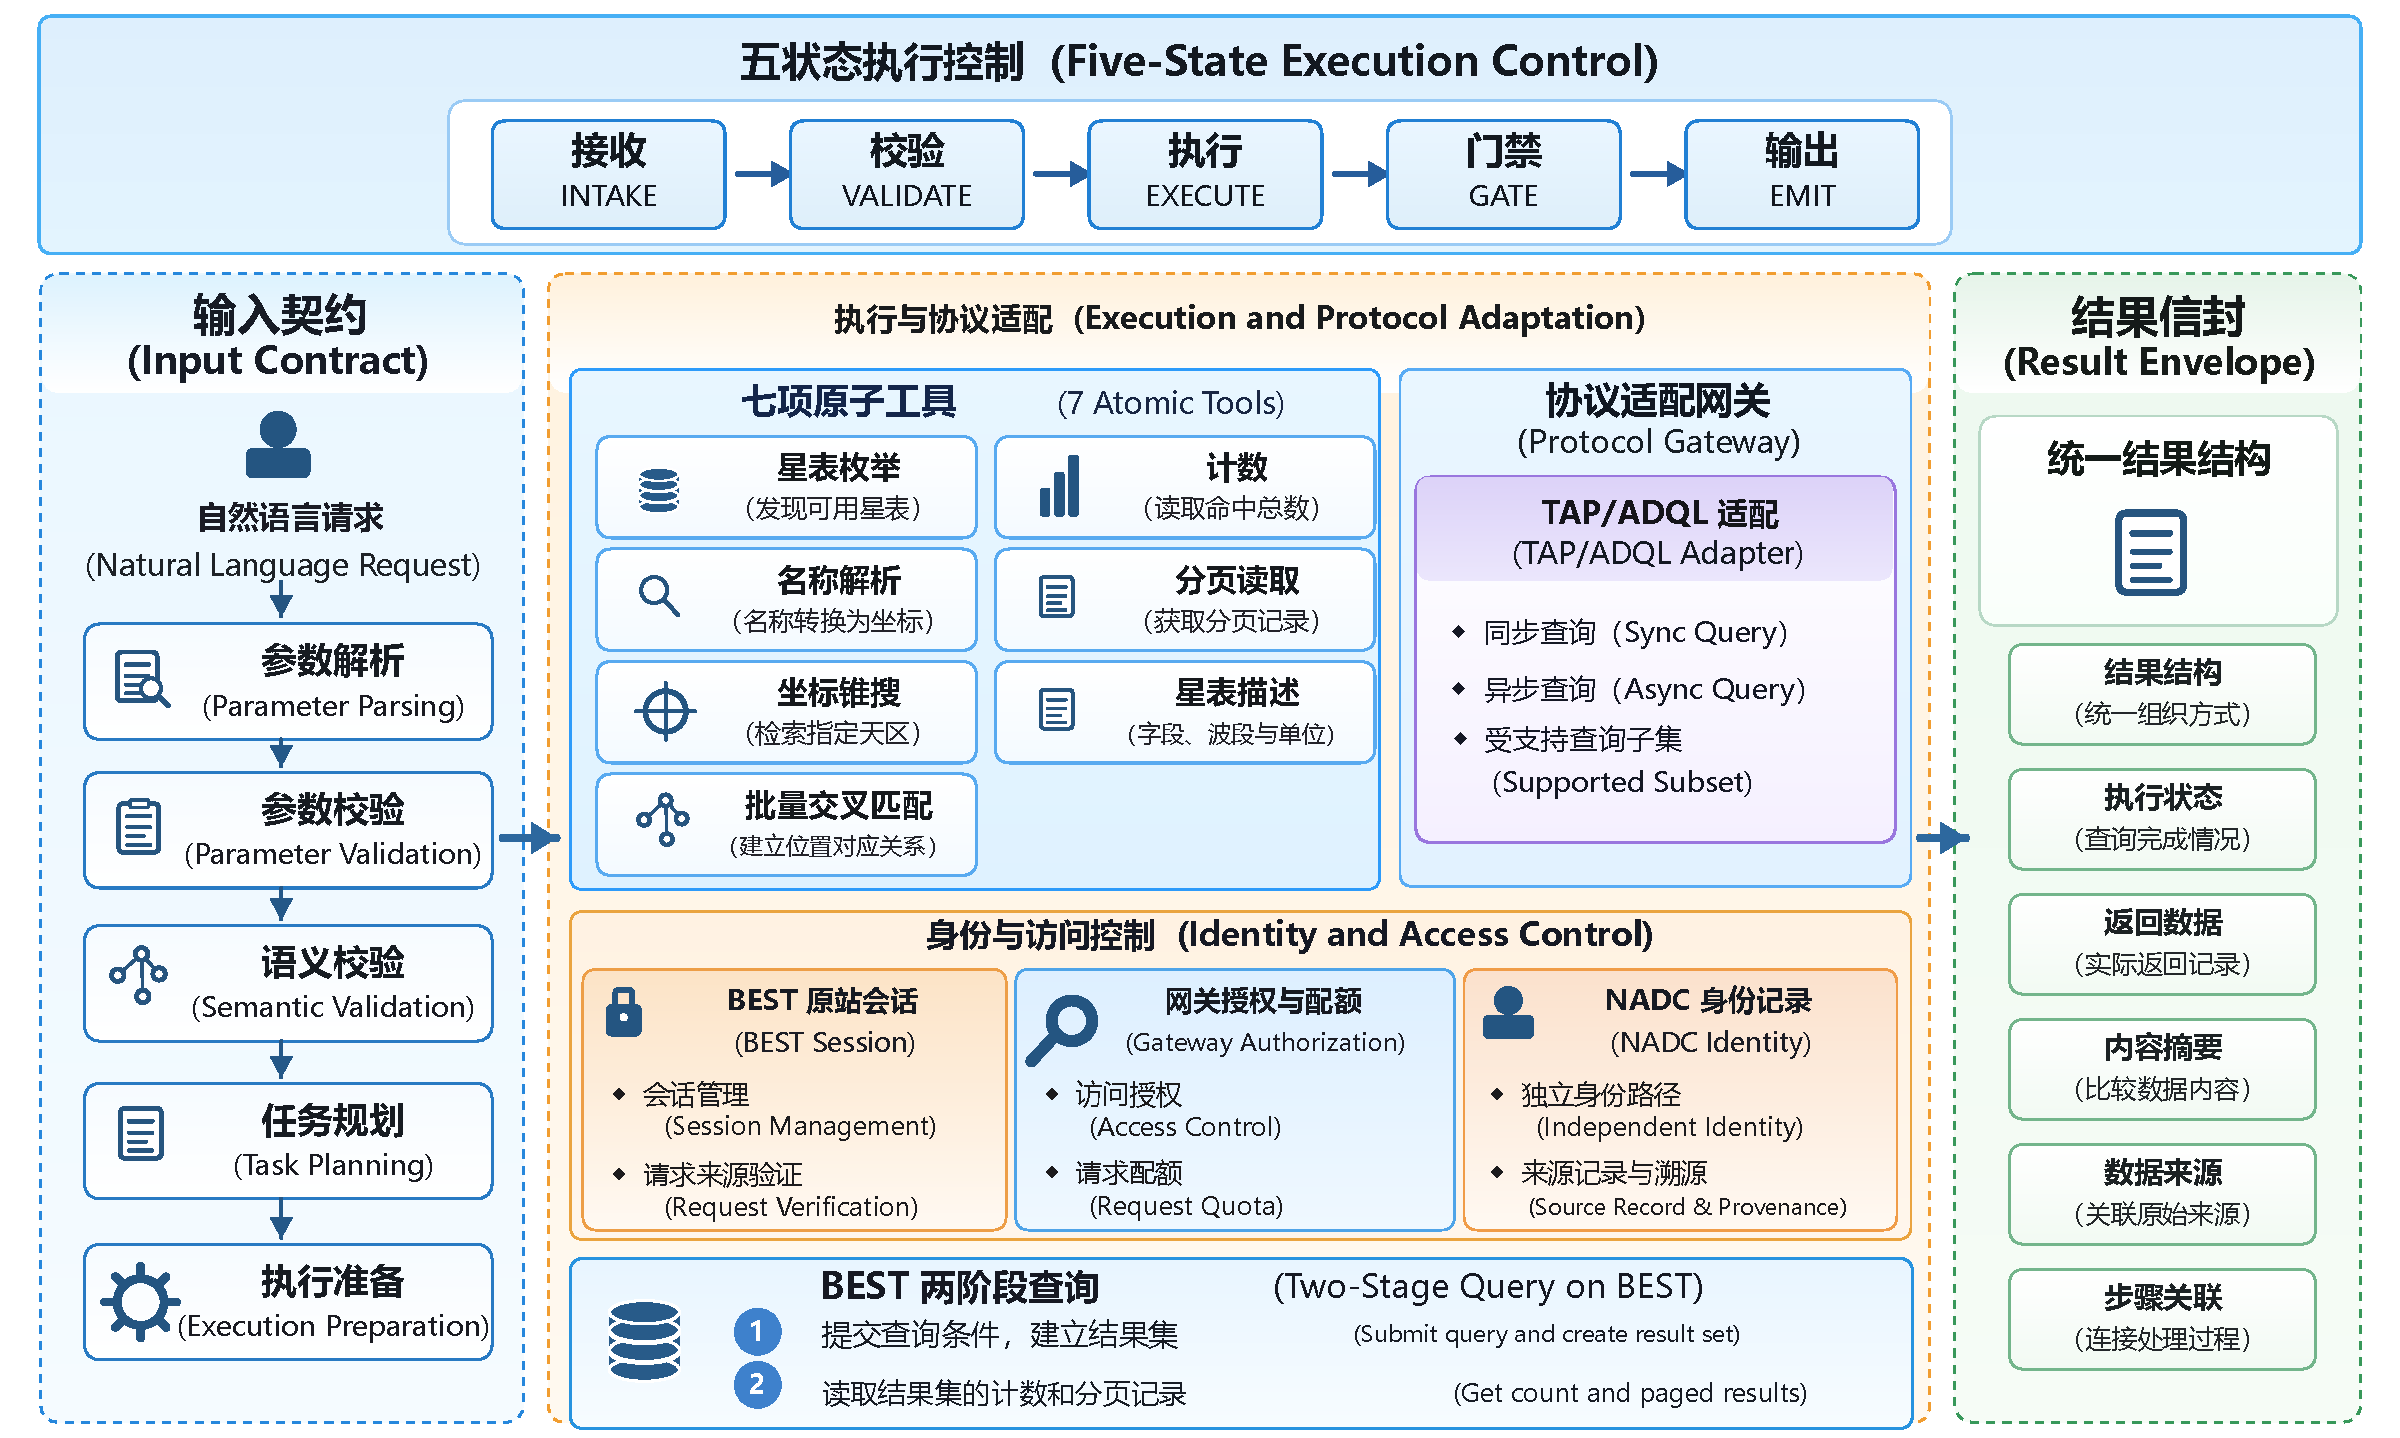
\includegraphics[width=\textwidth]{figures/fig1_architecture.pdf}
\figcaption{BEST-Skill 的访问接口与执行流程。七项原子工具（星表枚举、星表描述、名称解析、坐标锥搜、批量交叉匹配、结果计数和分页读取）；五状态机组织请求处理，TAP/ADQL 网关承接标准查询，统一结果信封交付数据、状态与来源}{Access interfaces and execution workflow of BEST-Skill. The seven tools support catalog listing and description, name resolution, cone search, batch cross-matching, result counting and pagination. The state workflow, TAP/ADQL gateway and result envelope organise execution and deliver data, status and provenance}
\label{fig:architecture}
\end{figure*}

智能体通过原子工具访问数据，标准协议客户端通过 TAP/ADQL 网关提交查询；两类入口连接同一 BEST 上游访问过程。原站会话维持数据库访问，网关授权控制访问权限与返回数量，用户身份记录用于关联数据来源。这样的分工使标准协议适配与具体数据操作保持衔接，同时便于分别管理原站访问和网关服务。

结果在单次操作和完整流程两个层面保存。前者记录某项操作返回了什么、是否完成以及数据来自何处；后者连接各步骤的输入与输出，形成可追溯的处理链。单次操作出现异常时，可以沿处理链定位其影响范围；多次操作共同完成查询时，也能保留从初始需求到最终数据的对应关系。具体接口与结果结构见补充材料附录 A.1—A.2；跨次运行的比较采用附录 A.3 给出的四项一致性指标。

\subsection{输入契约与参数校验}

接收阶段提取请求中的研究对象和查询条件，校验阶段依据输入契约检查坐标范围、半径单位、星表名称和可用字段。字段元数据中的缺测编码按缺测状态处理，原始测量值及其编码保留在返回记录中。图1中的语义校验指字段、单位及能力约定的契约检查，为请求理解、工具执行和结果解释提供可核对的依据；它不判断模型输出的全部科学主张是否成立。

请求按四类策略处置：A 类为确定性纠正，适用于含义唯一的单位转换等情形，声明纠正后继续；B 类为确定性拒绝，适用于非法或不支持的请求；C 类为请求澄清，适用于缺少单位、名称无法解析等情形；D 类为安全停止，适用于响应体为错误提示或查询状态无法确认等情形，停止并报告事实。合法直接回答作为单独类别统计。例如，负值角半径进入拒绝分支且不发起查询，缺少角半径单位的请求进入澄清分支，可唯一确定的角度单位换算则采用纠正。各类错误码及对应行为见补充材料附录 A.4。

\subsection{协议适配、查询执行与身份认证}

\subsubsection{原子工具与两阶段查询}

执行阶段调用七项原子工具，按访问准备、空间查询和结果读取组织如下：

\begin{enumerate}
\item 访问准备：星表枚举返回可用星表；星表描述返回字段、波段和单位，二者读取本地注册表而不产生站点请求。名称解析将天体名称转换为查询坐标，解析失败时提示更换名称或使用坐标入口。
\item 空间查询：坐标锥搜检索指定天球位置及角半径内的记录；批量交叉匹配对多个输入坐标进行位置匹配。批量执行保留每个条目的结果或失败状态，以便区分局部失败与整批失败。
\item 结果读取：计数读取已建立结果集的命中总数，分页读取按指定范围获取记录。二者使用同一查询结果集，使总记录数、已返回记录数和后续分页能够相互对应。各工具的具体接口、默认参数及异常处理见补充材料附录 A.1；能力组织与扩展接口见附录 A.5。
\end{enumerate}

两阶段查询将结果集的建立与读取分开。提交条件后，原站建立查询结果集；随后，计数和分页读取均围绕这一结果集进行。以坐标锥搜为例，系统先确定指定天区中的匹配记录，再读取命中总数并获取所需页面。若数据超过返回上限，输出中同时保留实际返回数量和截断状态，使调用方能够判断结果是否完整；若没有匹配记录，则报告查询完成和零条命中。由此，成功零行、查询失败和部分返回具有不同的结果含义。

\subsubsection{TAP/ADQL 协议适配}

本文在 BEST 原站之外实现 TAP 查询网关，提供同步、异步以及数据表描述等标准访问功能\citep{ref6}。网关将 ADQL 表达式解析为星表、所选字段、筛选条件和排序要求，再转换为原站能够执行的查询。查询完成后，原站返回的数据和状态按标准接口交付给客户端。该过程使采用国际虚拟天文台联盟（International Virtual Observatory Alliance，IVOA）标准的软件能够通过 TAP 和 ADQL 访问 BEST 数据\citep{ref6,ref13}，而无需理解原站的具体网页交互。

适配层支持字段选择、返回数量限制、条件筛选、排序和天球锥形查询。例如，在国际天球参考系（International Celestial Reference System，ICRS）下指定位置和角半径后，网关将空间约束与字段要求共同映射为原站查询条件。未覆盖的表达式在执行前返回明确说明，不向原站发起相应查询。结果数量超过请求上限时，保留截断信息；异步查询则允许客户端在提交后查询进度并读取结果。

\subsubsection{身份认证与凭据分离}

BEST 原站访问采用会话认证，并使用跨站请求伪造防护机制验证请求来源。客户端完成登录后，在后续查询中维持有效会话，使查询建立、计数和分页读取能够连续执行。

TAP 网关独立验证访问身份，并按授权范围配置返回数量和资源配额。身份认证决定客户端可以使用的服务范围，输入校验则判断当前科学请求是否满足执行条件。两者共同约束查询执行，避免将已获得访问权限等同于任意查询均可执行。

国家天文科学数据中心（National Astronomical Data Center，NADC）的身份服务通过开放授权协议 2.0（OAuth 2.0）提供可选用户身份记录，用于关联访问者与数据来源。原站会话、网关授权和身份记录分别承担数据访问、服务权限管理和来源关联职责，凭据由各自机制管理。

\subsection{结果封装与来源追溯}\label{sec:envelope}

查询执行后，系统检查结果是否完成、记录结构是否符合请求，以及实际返回数量是否与查询状态一致。检查通过后，将数据与相应的状态一并输出。对查询失败、成功零行和结果截断分别记录，使后续分析能够依据实际获得的数据继续处理。

统一结果信封将返回数据与查询条件、执行状态和数据来源关联，并记录上下游处理步骤之间的关系。为比较数据内容是否一致，系统保存由数据内容计算得到的摘要；为判断分页是否完整，则结合命中总数、已返回数量和截断状态进行检查。这些信息使后续分析既能使用查询结果，也能确认其范围与来源。具体结果结构见补充材料附录 A.2。

\section{评价设计与结果分析}

评价包含六组任务：E1 为工具映射评价，检验自然语言请求与工具及参数的对应关系；E2 为查询契约评价，检验固定场景下的字段、行集、分页和状态；E3 为科学语义忠实度评价，检验科学陈述与数据及其适用条件的一致程度；E4 为请求边界处置评价，检验 A—D 类及合法直接回答的处置；E5 为基线比较与指导信息消融评价；E6 为重复运行一致性评价，检验同一任务多次运行的稳定程度。

重复运行从工具序列、参数设置、返回数据和核心结论四个方面评价稳定性，分别记为工具选择一致性（Tool Selection Consistency，TSC）、参数一致性（Parameter Consistency，PAC）、返回数据一致性（Returned Data Consistency，RDC）和核心结论一致性（Final Core Conclusion Consistency，FCC）。其中 TSC 在本文以工具序列为比较对象，PAC 比较各次运行的调用参数并事先统一单位与字段限定方式、排除会话标识等易变值，RDC 比较规范化后的返回数据，FCC 比较由结论类别、关键数值、对象和限定语构成的结论卡；四项指标均以该任务内的众数序列、众数参数或众数结果为参照。各指标先在同一任务的有效重复之间比较，再按任务等权汇总；计算式及数据处理规则见补充材料附录 A.3。

科学语义比较中的 S-A 为提供完整访问机制和领域材料的配置，S-B 为基础包装器；E5 中 B2b 为原子工具基线，B3 在相同原子工具上增加完整指导信息。各组按相应任务及统计单位评价。表~\ref{tab:strata} 汇总各组材料、规模与解释范围；表~\ref{tab:claim-evidence} 明确研究主张与证据之间的对应关系。

\begin{columntable}
\tabcaption{研究主张、评价证据与结论范围}{Research claims, evaluation evidence and scope of conclusions}
\label{tab:claim-evidence}
\fontsize{8bp}{11bp}\selectfont
\begin{tabularx}{\linewidth}{@{}>{\RaggedRight\arraybackslash}p{0.29\linewidth}>{\RaggedRight\arraybackslash}p{0.23\linewidth}>{\RaggedRight\arraybackslash}X@{}}
\toprule
\textbf{研究主张} & \textbf{对应证据} & \textbf{结论范围} \\
\midrule
执行机制按约定处理数据与状态 & E2、协议故障测试 & 所测场景的契约符合性 \\
指导信息改善模型任务表现 & E5 的 B3—B2b 比较及指导消融 & 相同工具条件下的指导效果 \\
完整配置改善科学语义表达 & E3 的 S-A—S-B 比较 & 完整机制与领域材料的组合效果 \\
流程具有重复稳定性 & E6 & 固定回包与有效记录条件下的一致性 \\
\bottomrule
\end{tabularx}
\end{columntable}

\subsection{任务数据与评价指标}

\subsubsection{任务组织与数据处理}

评价材料覆盖自然语言查询、固定查询场景、科学解释题目、异常请求及重复运行任务。每项评价均预先确定输入条件、预期结果和评分依据，数据组织与分析流程见图~\ref{fig:data-model}。实站快照是从实际数据服务保存的响应；固定回包重放重复使用已保存的响应，以保持数据条件一致；合成压力数据用于考察分页与截断等边界行为。查询契约评价采用独立标准答案集作为参照，科学语义评价则依据预设关键科学断言评分。补充材料附录 B.1 提供 E1 题目，B.2—B.4 提供 E2 场景，B.5—B.6 提供 E3 题面与评分判据，B.7—B.8 提供 E4 场景，B.9 提供扩展任务模板，B.10 提供 E6 题目；补充统计与 E5 指导信息消融结果见附录 C。

\begin{figure*}[!t]
\centering
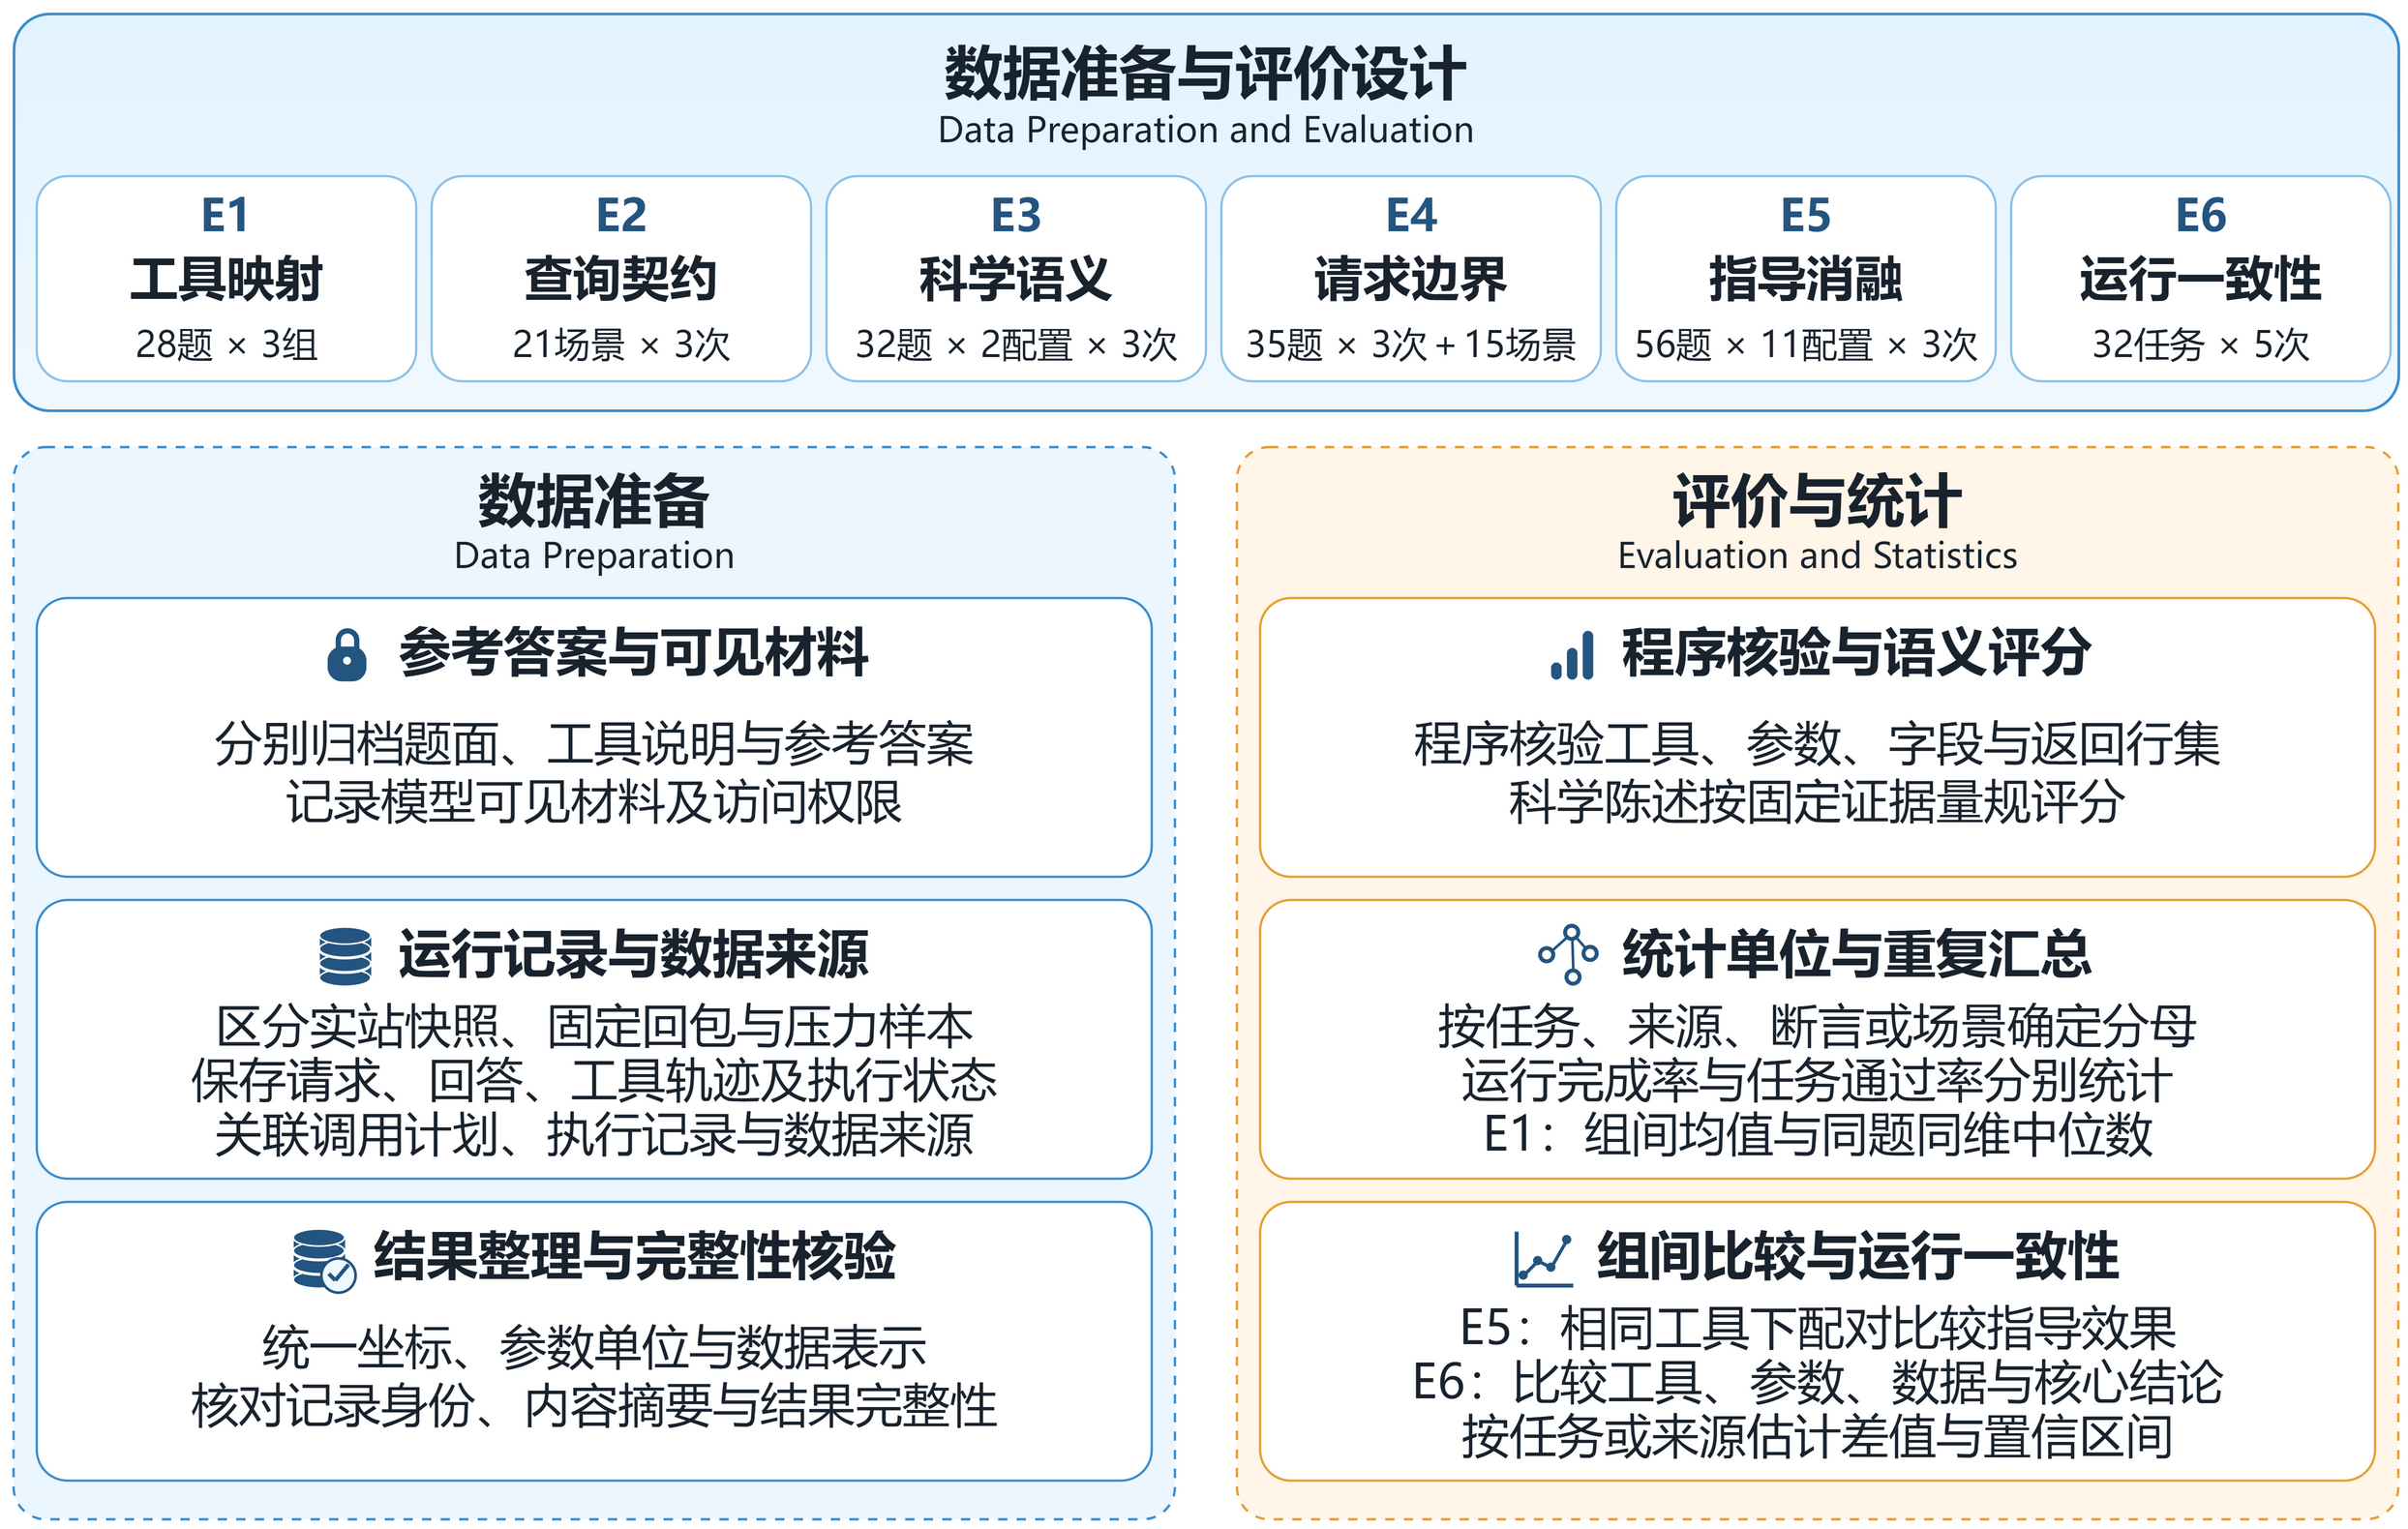
\includegraphics[width=0.96\textwidth]{figures/fig2_data_model.png}
\figcaption{BEST-Skill 的数据准备与评价设计：上方汇总六组评价任务与数据条件；左栏展示参考答案与可见材料、运行记录及结果完整性核验；右栏展示程序与语义评价、统计单位和运行一致性分析。}{Data preparation and evaluation design of BEST-Skill. The top row summarises the six evaluation groups and data conditions. The left column presents reference materials, execution records and result-integrity checks; the right column presents scoring, statistical units and consistency analysis.}
\label{fig:data-model}
\end{figure*}

\begin{columntable}
\tabcaption{各组评价材料、规模与主要判据}{Evaluation materials, sample sizes and primary criteria}
\label{tab:strata}
\fontsize{8bp}{11bp}\selectfont
\begin{tabularx}{\linewidth}{@{}>{\RaggedRight\arraybackslash}p{0.16\linewidth}>{\RaggedRight\arraybackslash}X@{}}
\toprule
\textbf{评价批次与维度} & \textbf{评价材料、判据与解释范围} \\
\midrule
E1 工具映射 & \textbf{材料与规模：}28 个任务（统计单位），三组回答，共 84 份答案\newline \textbf{主要判据：}工具、参数、转换、冗余、澄清及拒绝六维得分\newline \textbf{解释范围：}综合分与逐维指标共同验证请求映射质量（指导信息） \\
E2 查询契约 & \textbf{材料与规模：}21 个固定查询场景，每场景重复三次\newline \textbf{主要判据：}行集、字段、分页、状态与结果信封，逐项核对并与独立标准答案对照，任一项不符即判为不一致\newline \textbf{解释范围：}所测固定输入和响应条件下的查询契约符合性（执行机制） \\
E3 科学语义 & \textbf{材料与规模：}32 个题目（统计单位）×2 种配置×3 次重复；24 份在线辅助回答单列\newline \textbf{主要判据：}关键科学断言命中率、无来源科学数值率、无支撑科学主张率、必要限定语覆盖率与严格合格率\newline \textbf{解释范围：}完整访问机制与领域材料相对于基础包装器的组合效果（两层组合） \\
\bottomrule
\end{tabularx}
\end{columntable}

\begin{columntable}
\caption*{表~\ref{tab:strata}（续）\\Table~\ref{tab:strata} (continued)}
\fontsize{8bp}{11bp}\selectfont
\begin{tabularx}{\linewidth}{@{}>{\RaggedRight\arraybackslash}p{0.16\linewidth}>{\RaggedRight\arraybackslash}X@{}}
\toprule
\textbf{评价批次与维度} & \textbf{评价材料、判据与解释范围} \\
\midrule
E4 请求边界 & \textbf{材料与规模：}35 × 3 个自然语言请求场景全部计入整体处置正确率，其中适用加权判据的（18、21、16）个场景另计加权分；15 个协议故障场景按预设错误码逐条核验\newline \textbf{主要判据：}纠正、拒绝、澄清、停止报告与合法直接回答的处置正确率\newline \textbf{解释范围：}整体处置与加权判据分别统计并给出通过率（自然语言请求属指导信息；协议故障属执行机制） \\

E5 基线与指导消融 & \textbf{材料与规模：}56 题（统计单位）、11 种配置、每题三次，共 1848 次运行；另设交叉匹配扩展评价\newline \textbf{主要判据：}端到端规则通过率、工具调用与输出 token\newline \textbf{解释范围：}分级基线比较；同工具条件下指导信息的影响（指导信息） \\
E6 重复运行 & \textbf{材料与规模：}32 个任务×5 次计划运行，共 160 次运行\newline \textbf{主要判据：}有效记录率及工具序列、参数设置、返回数据与核心结论的一致性\newline \textbf{解释范围：}固定回包下报告有效记录比例及有效重复间一致性（流程稳定性） \\
\bottomrule
\end{tabularx}
\end{columntable}


科学语义评价包含 32 个独立题目。完整配置和基础包装器对每题分别生成三次回答，共获得 192 份离线主测回答；在线辅助评价包含 4 个题目，共 24 份回答。查询契约评价包括 21 个固定场景，每个场景重复三次。重复运行评价对 32 个任务分别执行五次；具有完整回答及所需运行记录的结果计为有效记录，符合要求的澄清或拒绝也计入其中。

\subsubsection{评价指标与统计方法}

工具映射评价依据统一量规评价工具选择、参数正确性、单位与坐标转换、冗余控制、澄清和拒绝六个维度，其中工具集合匹配采用 F1 分数，即实际工具集合与预期工具集合交集大小的两倍除以两个集合大小之和；六维权重依次为 0.30、0.25、0.15、0.10、0.10 和 0.10。各维度按适用任务汇总，再按上述权重计算总分。查询契约评价以独立标准答案为参照，比较返回记录、字段取值、分页和执行状态。科学语义评价以关键科学断言命中率为主指标，即命中的关键断言数占预设关键断言总数的比例。辅助指标包括无来源科学数值率（无来源数值数/回答中数值总数）、无支撑科学主张率（无支撑主张数/科学主张总数）、静态测光数据的时间序列误述率（误述题数/涉及时序语义的题数）、必要限定语覆盖率（已给限定语数/应给限定语数），以及严格合格率（全部关键断言命中、无禁答冲突且无严重科学错误的题目比例）。必要限定语指题目要求保留的来源、测光系统、缺失值及适用子集等条件。严重科学错误按评分量规中预设的错误类型判定，具体条目见补充材料 B.6。请求边界评价分别统计协议故障场景、自然语言请求场景和适用加权判据场景的处置结果。重复运行评价同时统计有效记录比例及有效重复之间的一致性。

科学语义评价中的三次重复指标以中位数汇总。每组每次重复包含 71 条关键科学断言、73 条必要限定语和 14 道涉及时序语义的题目；严格合格率以 32 个题目为分母。组间差值的 95\% 置信区间（confidence interval，CI）按配对题号进行成组自助重抽样（bootstrap，即有放回地抽取任务并重算统计量）10000 次估计，同题多次回答不作为独立题目。逐题三次重复多数判定后的配对二分类结果使用双侧精确 McNemar 检验，以不一致对的二项分布计算概率\citep{ref14,ref15}。E5 基线与消融分析先在同题同配置内对三次重复取均值，再按题进行精确配对符号翻转检验。科学语义依据预设证据量规逐条评分，数值、参数、行集等可结构化字段由程序核验。各指标按其定义对应的断言、题号或限定语计算，统计单位见上述指标定义，同题重复回答按预设汇总方式处理。

重复运行分析先统一参数单位和数据表示，再比较各任务中的工具序列、参数设置、返回数据与核心结论。一致性估计纳入至少具有两次有效重复的任务，置信区间按任务成组重抽样 10000 次获得。

\subsection{评价配置与实现条件}

\subsubsection{运行环境与生成参数}

实验使用 deepseek-v4.1-flash 模型。科学语义与重复运行评价的推理强度设为最高，最大输出长度为 32768 个 token（模型处理和生成文本的计量单元），未主动指定温度和随机种子。E1 依据三组模型回答中的工具调用计划、参数与处置内容进行评价。E5 基线与消融评价为各配置设置相同的 4096 个最大输出 token，并使用相同的冻结公开响应；交叉匹配扩展评价采用相同模型，两组均设置 393216 个最大输出 token 及 180 秒期限。token 上限表示每次生成请求的预算，而非实际输出长度。数据采集与统计分析采用 Python。科学语义评价的两种配置采用相同生成参数；重复运行评价固定提示和工具实现，工具数据采用预先保存的 BEST 响应进行重放。

\subsubsection{对照配置与查询条件}

科学语义评价采用两种对照配置：完整配置（S-A）提供 BEST-Skill 的完整访问机制及领域材料；基础包装器（S-B）提供表名、列名和两阶段协议说明。两组使用相同题号与数据条件。S-A 与 S-B 的比较反映完整访问机制及领域材料相对于基础包装器的组合效果，不能单独归因于某项指导信息或执行机制。

查询契约评价场景覆盖实站快照、固定回包重放和边界测试。PS1（Pan-STARRS1 巡天）星表密集场使用 1000 行实站快照；60000 行压力数据由固定规则生成，用于检验 60 个分页、50000 行返回上限及截断标记；空值—零值对照用于区分原始空值、数值零与缺失值占位符。不同场景分别对应真实数据访问、固定条件复现和边界语义核验。

\subsection{结果分析}

\subsubsection{工具映射结果}

E1 包含 28 个任务与三组模型回答，共 84 份答案。三组加权分分别为 0.9429、0.9607 和 0.9554，均值为 0.9530，样本标准差为 0.0092，均高于 0.90 的总分参考线。六维得分均值为：工具集合匹配 0.9405、参数正确率 0.9659、单位转换正确率 1.0000、冗余调用控制 0.9881、澄清 0.8333、拒绝 0.9722。单位转换在三组均得满分，工具选择、参数映射与冗余控制亦保持较高水平。

对同题同维的三份回答先取中位数，再按维度汇总并加权，得到 0.9750；该值与三组均值 0.9530 分别描述稳健汇总表现与组间平均表现。澄清得分为 0.8333，说明确定查询条件之前识别必要追问仍是主要改进方向。图~\ref{fig:e1} 展示三组均值，表~\ref{tab:e1} 列出两种汇总口径。

\begin{columnfigure}
\centering
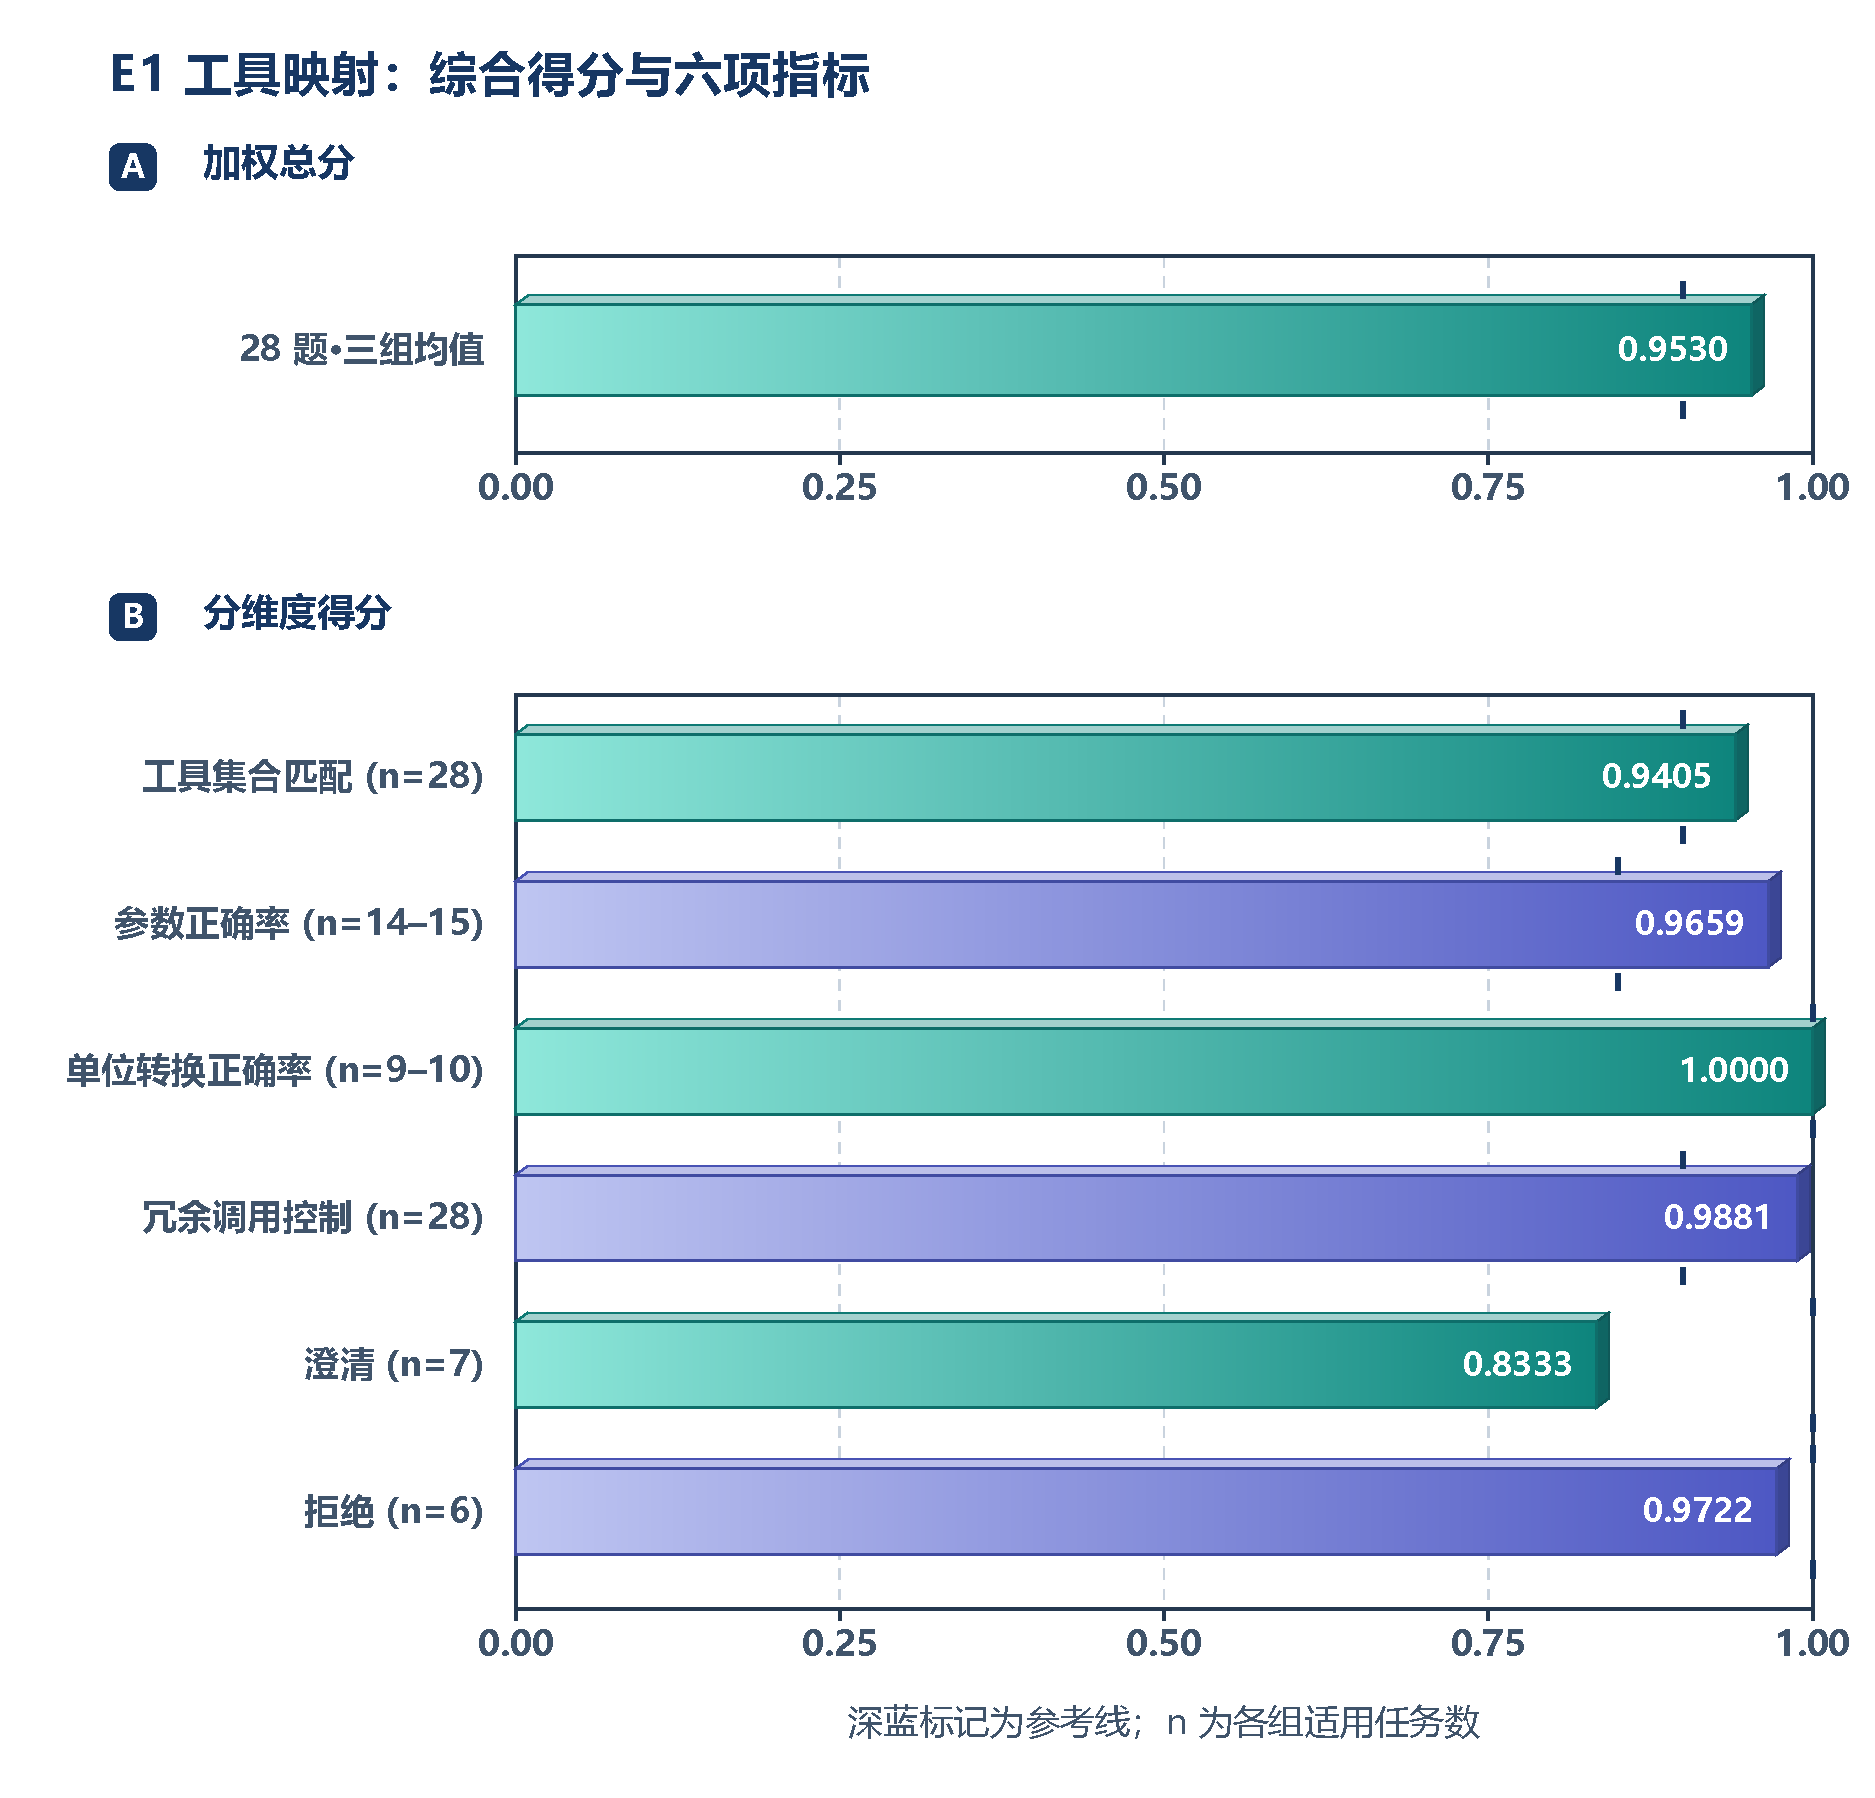
\includegraphics[width=\linewidth]{figures/fig3_e1.pdf}
\figcaption{E1 三组回答的平均得分；A 为加权总分均值，B 为六维均值，深蓝标记表示参考线；适用任务数可随回答组变化}{E1 mean scores across three answer sets; panel A shows the mean weighted score and panel B the dimension means; dark-blue marks show reference thresholds}
\label{fig:e1}
\end{columnfigure}
\begin{columntable}
\tabcaption{工具映射评价的两种汇总口径}{Two aggregation schemes for the tool-mapping evaluation}
\label{tab:e1}
\fontsize{8bp}{10.5bp}\selectfont
\begin{tabularx}{\linewidth}{@{}>{\RaggedRight\arraybackslash}p{0.245\linewidth} >{\RaggedRight\arraybackslash}p{0.180\linewidth} >{\RaggedRight\arraybackslash}p{0.170\linewidth} >{\RaggedRight\arraybackslash}X@{}}
\toprule
\textbf{指标} & \textbf{三组均值} & \textbf{中位汇总} & \textbf{参考线；适用任务数} \\
\midrule
加权总分 & 0.9530 & 0.9750 & 0.90；28 题 \\
工具集合 & 0.9405 & 0.9643 & 0.90；$n=28$ \\
参数 & 0.9659 & 1.0000 & 0.85；$n=14$--15 \\
单位转换 & 1.0000 & 1.0000 & 1.00；$n=9$--10 \\
冗余控制 & 0.9881 & 1.0000 & 0.90；$n=28$ \\
澄清 & 0.8333 & 0.8571 & 1.00；$n=7$ \\
拒绝 & 0.9722 & 1.0000 & 1.00；$n=6$ \\
\bottomrule
\end{tabularx}
\end{columntable}

\subsubsection{查询结果契约验证}

查询契约评价通过固定查询场景检验 BEST-Skill 对字段结构、结果行集、分页、查询状态与来源信息的处理。21 个固定场景各重复三次，63 次运行均完成，21 个场景均达到预设通过条件。场景覆盖密集星表查询、分页与截断、缺失值和数值零的区分，以及查询成功但无匹配记录等边界条件；各场景的标准答案由独立实现核验。

高密度 PS1 场景使用 1000 行、覆盖 0.7854 平方度的实站快照。分页压力场由固定规则生成 60000 行测试数据，按每页 1000 行对应 60 页完整数据，并设置 50000 行返回上限（最多返回 50 页数据）；相应判据要求结果同时保留总记录数、已返回行数和截断标记。空值—零值对照分别标记原始空值、数值零和缺失值占位符，确保它们在结果结构和后续计算中保持不同语义。上述场景将查询契约具体化为可逐项核验的字段与状态条件。

\begin{columntable}
\tabcaption{查询结果契约核验结果}{Query-contract verification results}
\label{tab:e2}
\fontsize{8bp}{10.5bp}\selectfont
\begin{tabularx}{\linewidth}{@{}>{\RaggedRight\arraybackslash}p{0.29\linewidth} >{\RaggedRight\arraybackslash}p{0.22\linewidth} >{\RaggedRight\arraybackslash}X@{}}
\toprule
\textbf{核验场景} & \textbf{结果} & \textbf{对应的契约属性} \\
\midrule
固定查询场景 & 21/21 通过 & 字段结构、行集与状态一致性 \\
密集星表快照 & 1000 行 & 真实数据条件下的结果结构核验 \\
分页压力场 & 60000 行，60 页 & 总数、返回上限、分页与截断标记 \\
空值—零值对照 & 三类取值分别标记 & 空值、数值零与缺失值编码的语义区分 \\
重复运行 & 63/63 完成 & 21 个场景，每场景三次 \\
\bottomrule
\end{tabularx}
\end{columntable}

\subsubsection{科学语义忠实度比较}

按预设评分量规汇总，完整配置 S-A 的关键科学断言命中率为 90.14\%，基础包装器 S-B 为 66.20\%，差值为 23.94 个百分点；配对题号自助法 95\% 置信区间为 12.68--33.33 个百分点。严格合格率的双侧精确 McNemar 检验为 $p=0.00049$。结果显示，完整访问机制在科学陈述与数据证据的对应关系上具有更高的评分表现。图~\ref{fig:e3} 与表~\ref{tab:e3} 汇总主要指标。

辅助指标显示，无来源科学数值率由 15.68\% 降至 7.14\%，无支撑科学主张率由 42.73\% 降至 30.26\%，必要限定语覆盖率由 87.67\% 提高至 95.89\%；静态测光数据的时间序列误述率由 14.29\% 降至 0\%，严格合格率由 40.62\% 提高至 81.25\%。这些指标分别评价数值来源、科学主张支撑、限定条件保留与数据类型解释。

\begin{columnfigure}
\centering
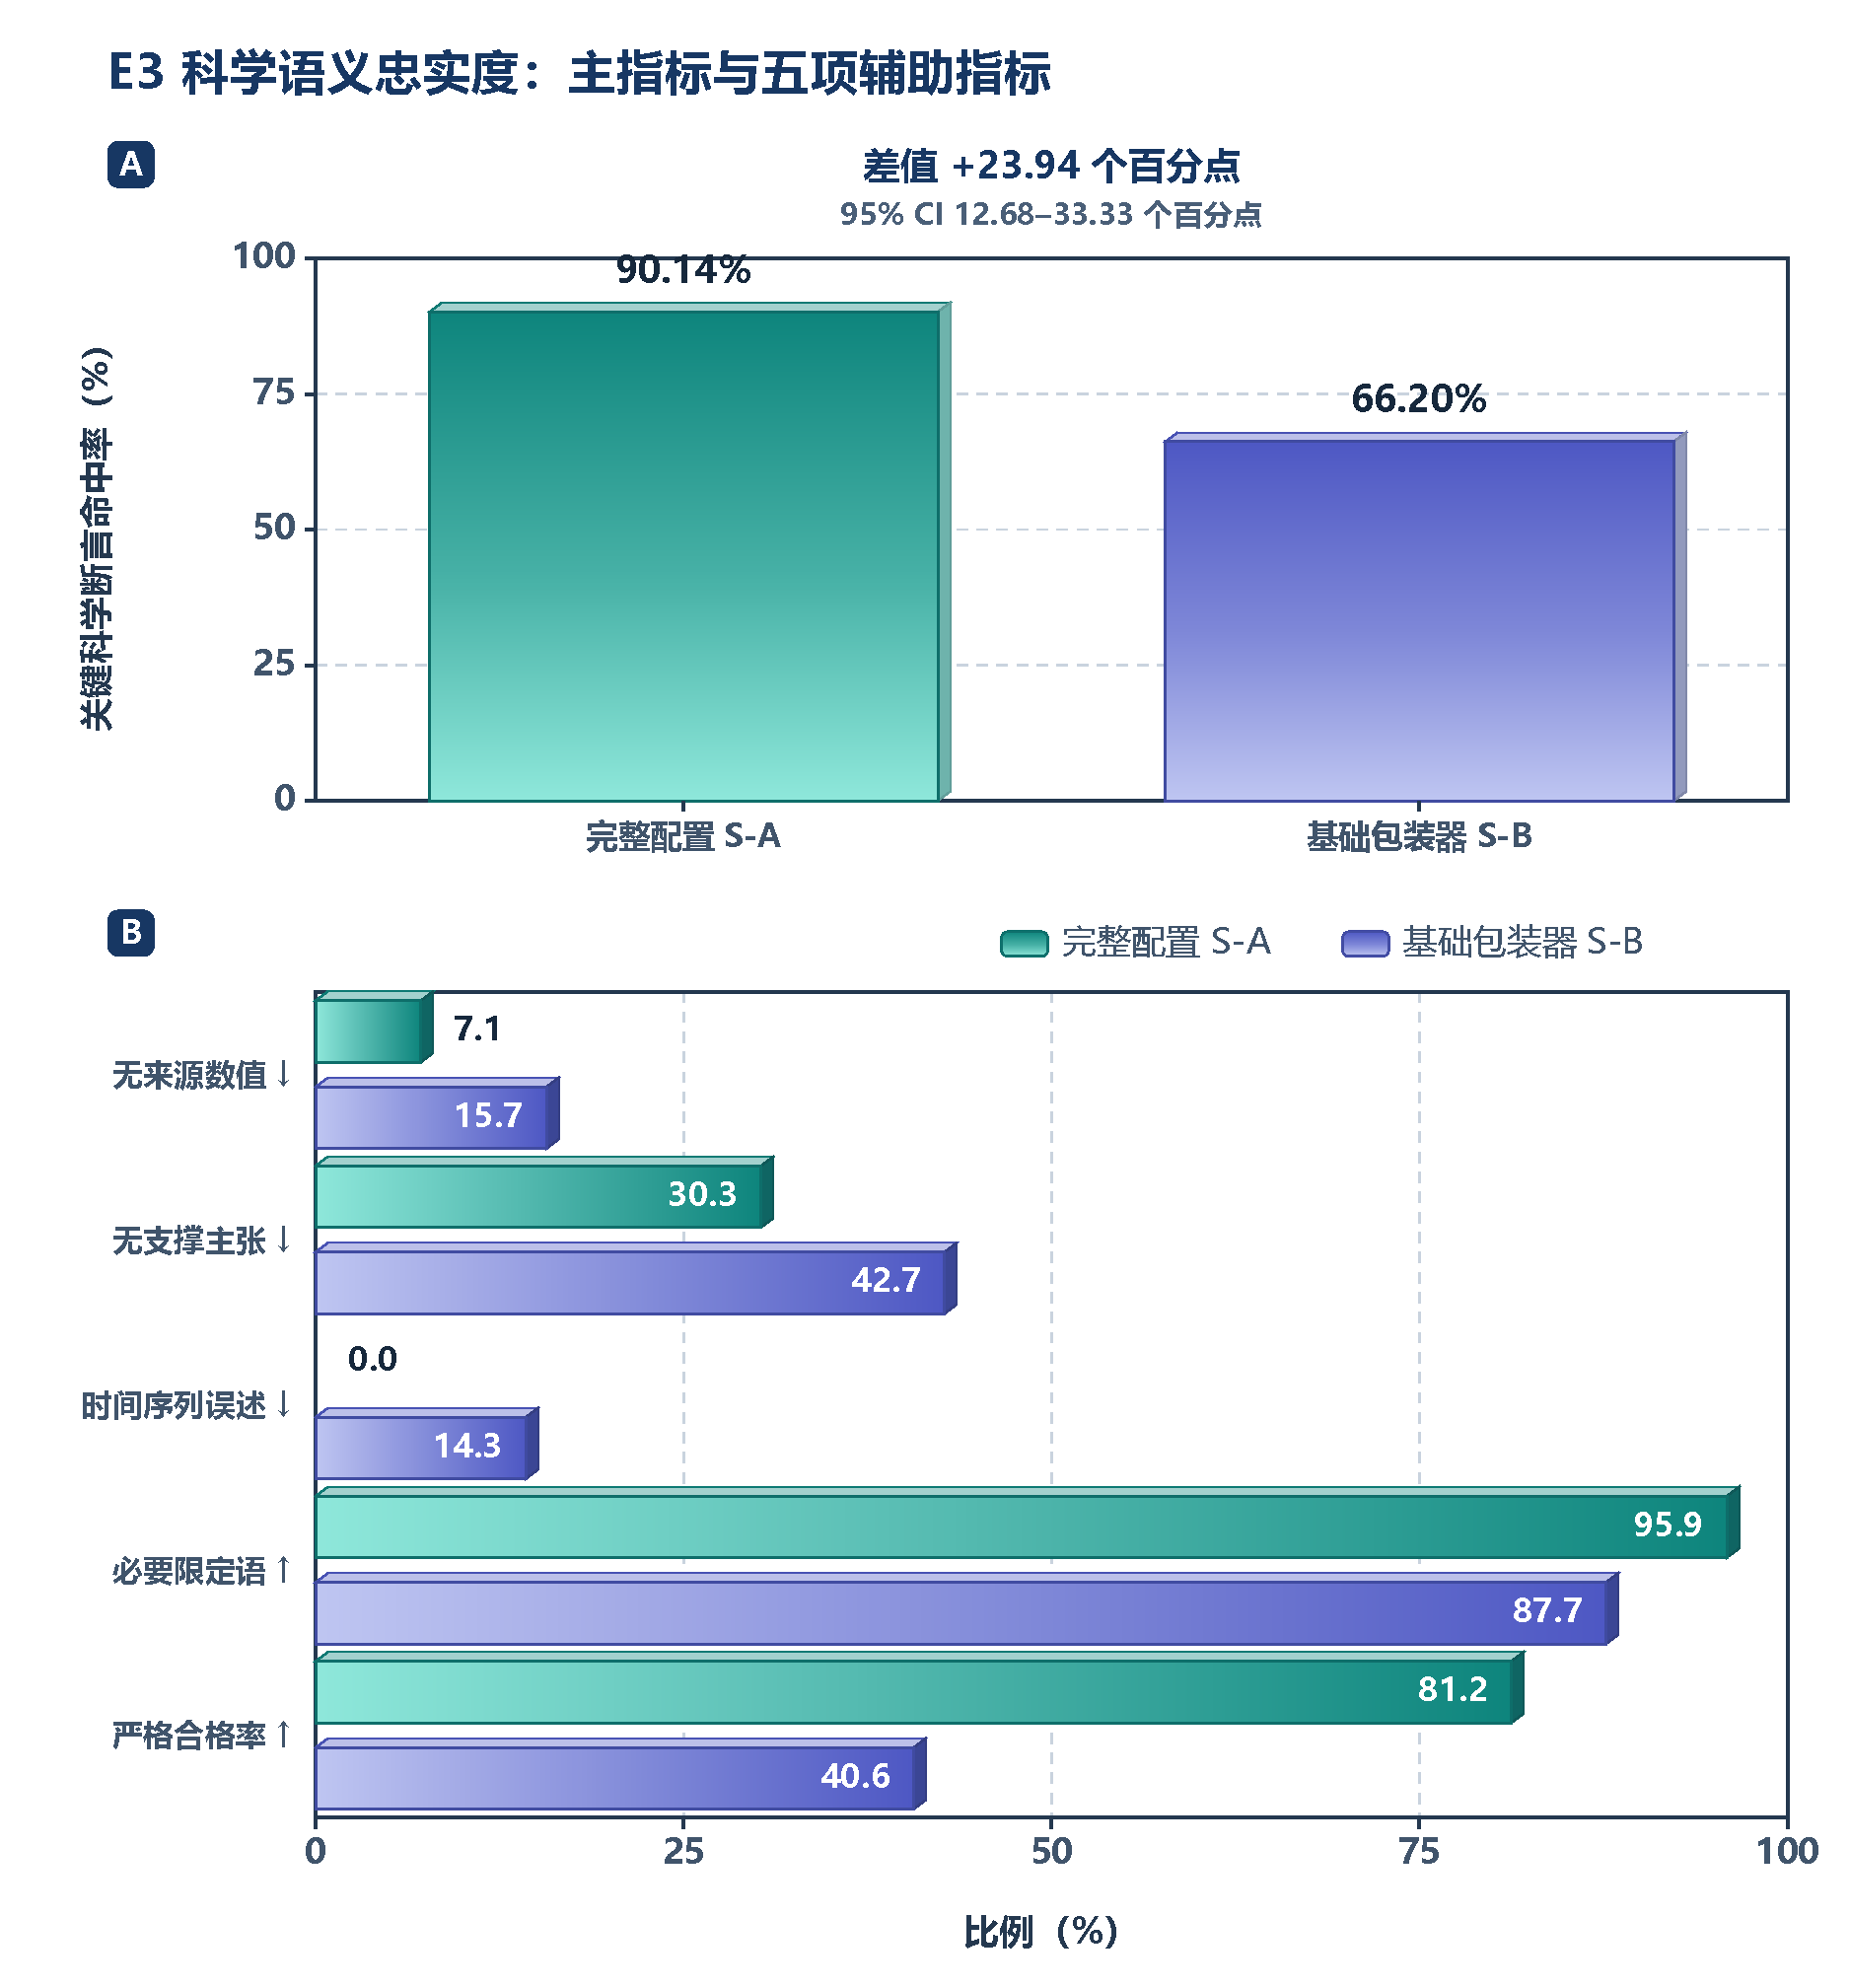
\includegraphics[width=\linewidth]{figures/fig4_e3.pdf}
\figcaption{科学语义忠实度比较：完整配置 S-A 与基础包装器 S-B 的关键科学断言命中率及辅助指标；A 为关键科学断言命中率，B 为五项辅助指标；时间序列误述率以涉及时序语义的题目为分母}{Scientific-semantic faithfulness for S-A and S-B. Panel A shows critical-assertion recall and panel B five auxiliary metrics; the temporal-misdescription rate uses time-related items as its denominator}
\label{fig:e3}
\end{columnfigure}

\begin{columntable}
\tabcaption{科学语义忠实度主要结果}{Primary results for scientific-semantic faithfulness}
\label{tab:e3}
\fontsize{8bp}{10.5bp}\selectfont
\begin{tabularx}{\linewidth}{@{}>{\RaggedRight\arraybackslash}p{0.240\linewidth} >{\RaggedRight\arraybackslash}p{0.240\linewidth} >{\RaggedRight\arraybackslash}p{0.440\linewidth}@{}}
\toprule
\textbf{指标} & \textbf{基础包装器 S-B} & \textbf{完整配置 S-A} \\
\midrule
关键科学断言命中率 & 66.20\% & 90.14\% \\
差值（S-A−S-B） & — & 23.94 个百分点 \\
静态测光数据的时间序列误述率 & 14.29\% & 0\% \\
严格合格率 & 40.62\% & 81.25\% \\
\bottomrule
\end{tabularx}
\end{columntable}

\subsubsection{请求边界与故障处置}

请求边界评价从协议故障与自然语言请求两个层面评价请求处置。自然语言请求评价的整体处置正确率为 （34/35、35/35、34/35）（97.14\%、100\%、97.14\%），适用加权判据的（18、21、16）个场景中有（8、13、10）个达到通过条件（44.44\%、61.90\%、62.50\%）。按类别统计，A 类为（3/3、3/3、3/3），B 类为（17/17、17/17、17/17），C 类为（9/9、9/9、9/9），D 类为（4/5、5/5、4/5），合法直接回答为（1/1、1/1、1/1）。类别之间的结果差异表明，请求处置既需要对输入约束进行明确判定，也需要结合自然语言语境识别应纠正、拒绝、澄清或停止的情形。协议单点故障场景的结果为 15/15 按预设规则处置；诱导话术子类为 5/5 处置正确。

\begin{columnfigure}
\centering
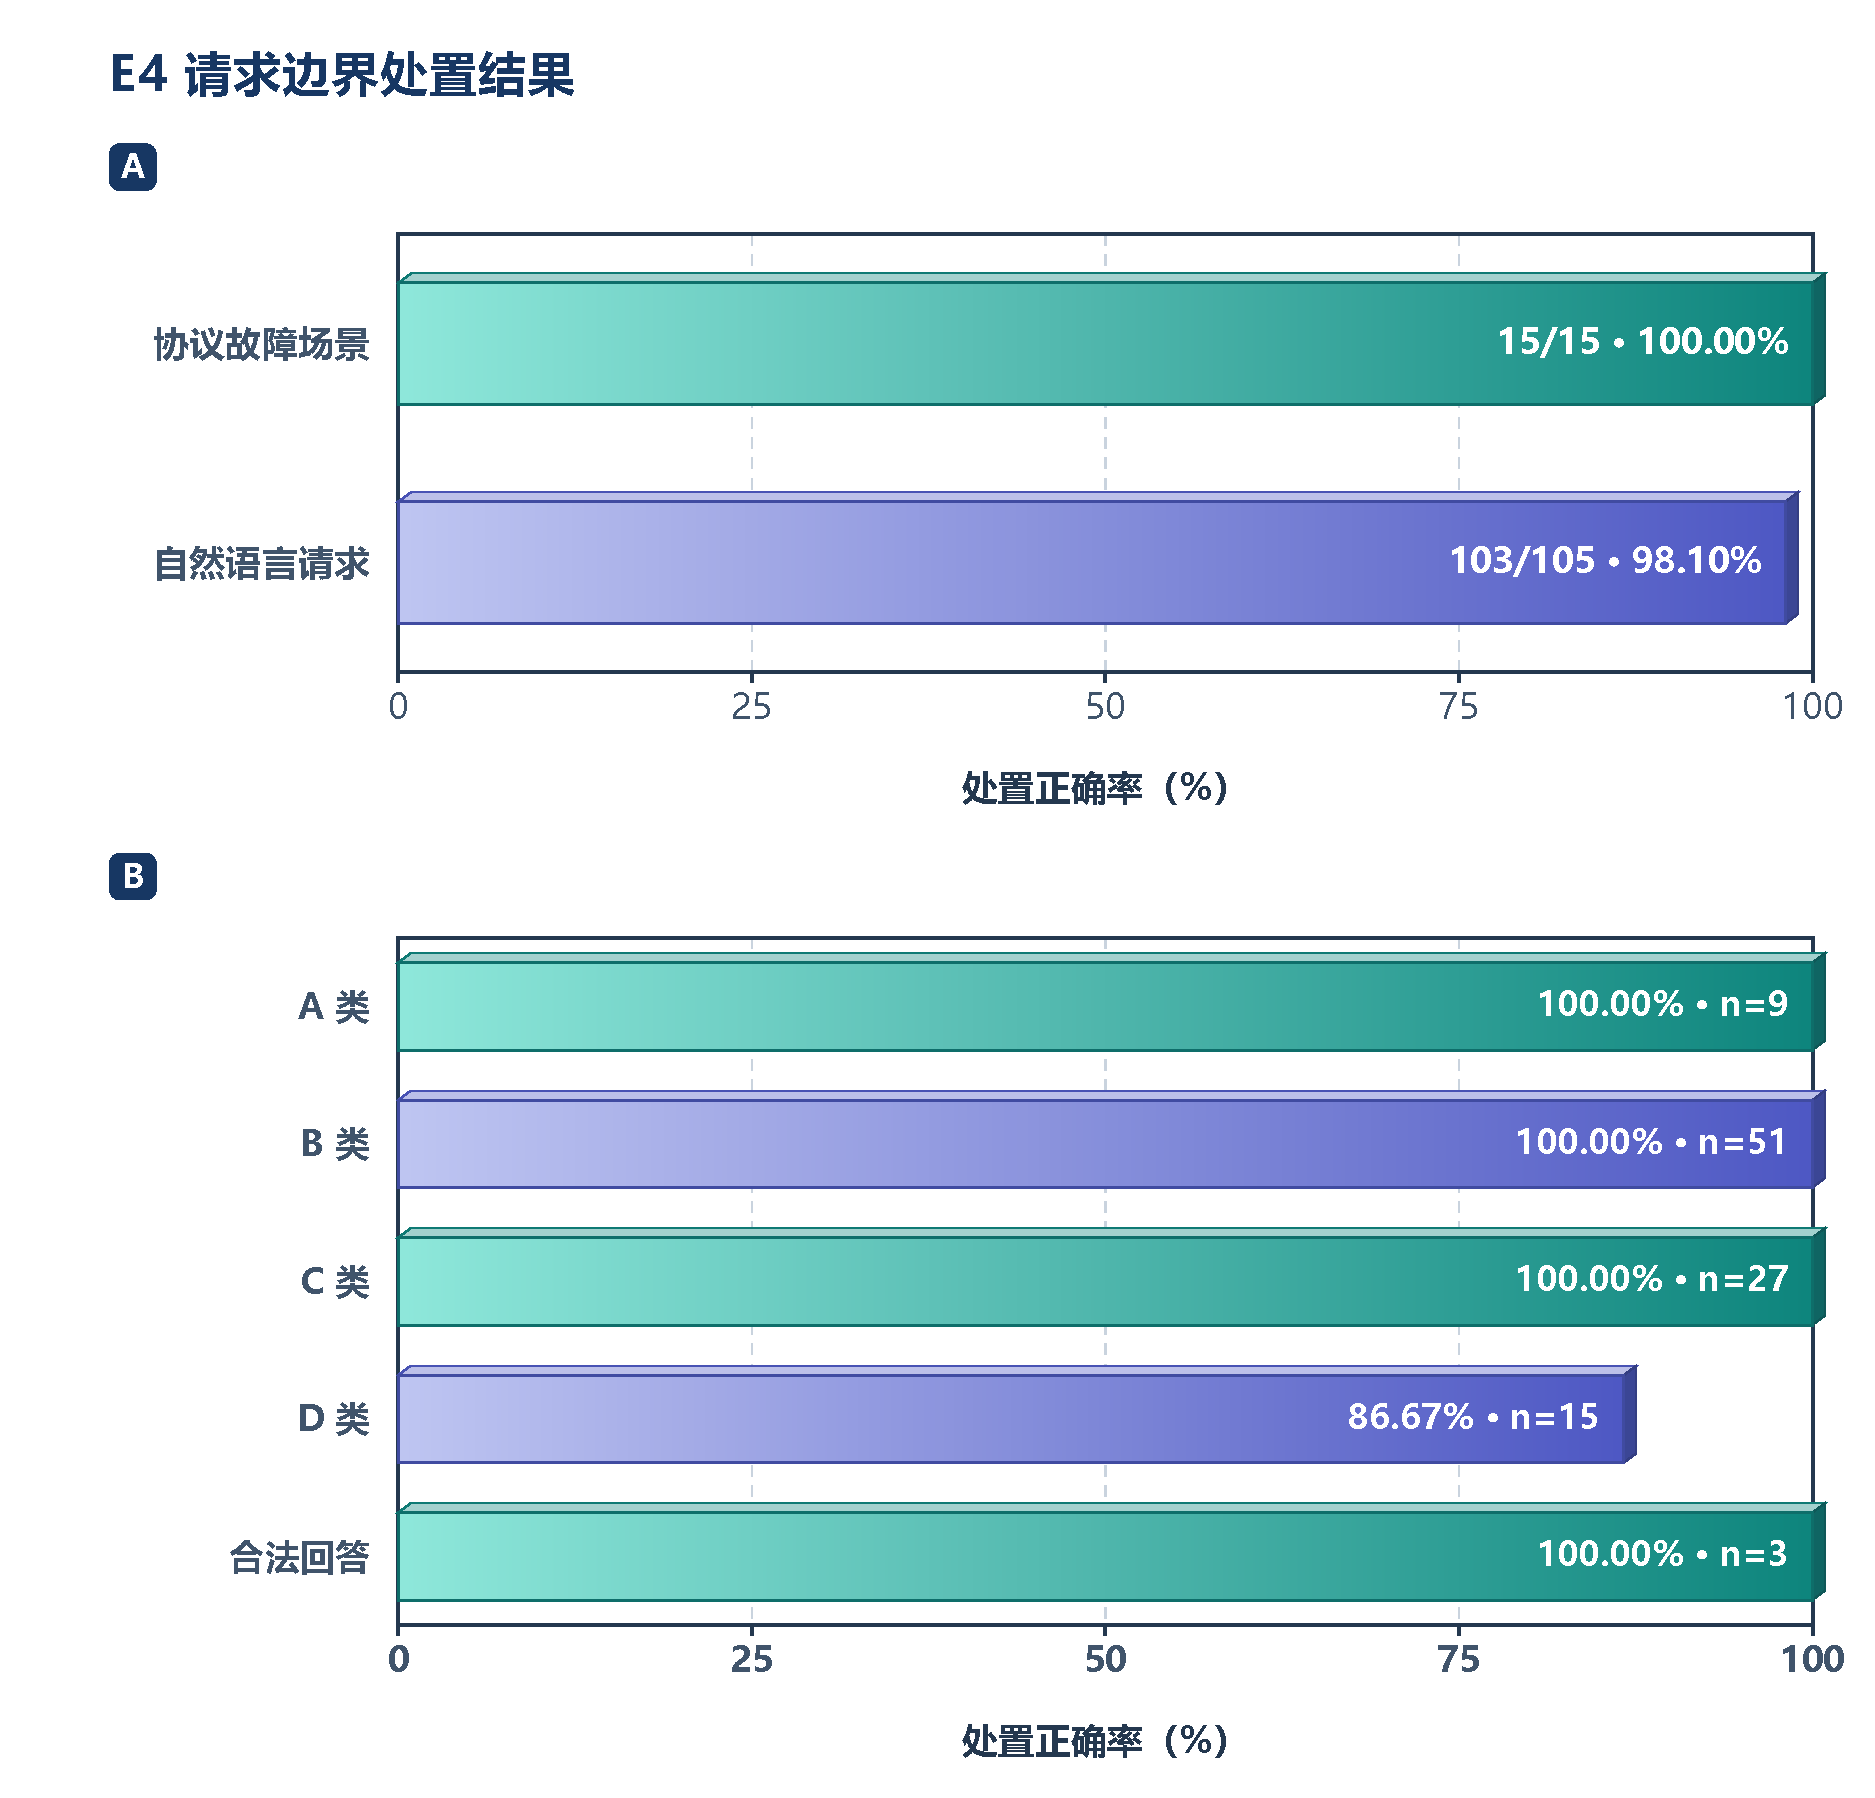
\includegraphics[width=\linewidth]{figures/fig5_e4.pdf}
\figcaption{请求边界处置结果：协议故障场景与自然语言请求评价的整体正确率，以及自然语言请求按处置类别划分的结果}{Request-boundary disposition: overall accuracy for protocol-fault scenarios and natural-language request scenarios, with category-level results for those scenarios}
\label{fig:e4}
\end{columnfigure}

\begin{columntable}
\tabcaption{请求边界处置结果}{Request-disposition results}
\label{tab:e4}
\fontsize{8bp}{10.5bp}\selectfont
\begin{tabularx}{\linewidth}{@{}>{\RaggedRight\arraybackslash}p{0.260\linewidth} >{\RaggedRight\arraybackslash}p{0.300\linewidth} >{\RaggedRight\arraybackslash}X@{}}
\toprule
\textbf{评价部分} & \textbf{结果} & \textbf{评价对象} \\
\midrule
协议故障场景 & 15/15 & 预设协议规则的处置 \\
自然语言请求处置 & \shortstack[l]{34/35（97.14\%）\\35/35（100\%）\\34/35（97.14\%）} & 自然语言请求的处置标签 \\
加权判据通过率 & \shortstack[l]{8/18（44.44\%）\\13/21（61.90\%）\\10/16（62.50\%）} & 适用加权判据的场景 \\
\bottomrule
\end{tabularx}
\end{columntable}

\subsubsection{基线比较与指导信息消融}

为区分文档、数据库接入与指导信息的贡献，E5 在相同的 56 个任务上比较四级基线，每种配置运行三次。B0 仅使用通用模型；B1 增加 BEST 文档但不提供查询工具；B2 提供数据库访问，其中 B2a 通过原始 API、B2b 通过原子工具访问；B3 在与 B2b 相同的原子工具基础上增加字段语义、参数校验、能力边界、来源信息与结果检查等指导信息。本文汇总五种基线实现与六种消融配置，合计 11 种配置、1848 次模型运行。所有配置使用相同题面、模型及生成预算。端到端规则通过率要求该题的决策、操作、引用与回答同时满足预设条件，由程序按预设规则自动计分。

E5 的指导信息消融在共享工具实现和硬性执行约束保持一致的条件下，移除不同类别的模型指导信息。因此，该实验估计的是指导信息对模型行为与任务表现的影响，不用于估计相应程序执行机制的独立贡献。执行机制的契约符合性由 E2 固定场景测试及协议故障测试另行评价。B0、B1 与 B2a 用于分级基线描述，指导层的同工具主比较为 B3 与 B2b。

在四级基线中，B3 的端到端规则通过率最高，为 95/168（56.55\%），B0、B1、B2a 和 B2b 分别为 17.26\%、26.19\%、48.81\% 和 49.40\%（表~\ref{tab:e5}）。相对 B0、B1 和 B2a，B3 的通过率分别高 39.29、30.36 和 7.74 个百分点。这一递增趋势表明，数据库接入对应较大的总体表现差异；在已具备数据访问能力后，额外指导信息呈正向总体差值。

在相同原子工具条件下，B3 相较 B2b 的规则通过率高 7.14 个百分点。B3 的平均工具调用次数由 7.23 降至 4.85，减少 32.95\%；每次任务运行的输出 token 合计均值由 4036.8 降至 3534.8，减少 12.44\%。

\begin{columntable}
\tabcaption{E5 四级基线的规则通过率与运行开销}{Rule-based pass rates and execution overhead across the four E5 baseline levels}
\label{tab:e5}
\fontsize{8bp}{10.5bp}\selectfont
\begin{tabularx}{\linewidth}{@{}lXXX@{}}
\toprule
\textbf{配置} & \textbf{通过率} & \textbf{平均调用} & \textbf{输出 token} \\
\midrule
B0 & 17.26\% & 0.00 & 1372.9 \\
B1 & 26.19\% & 0.00 & 1560.9 \\
B2a & 48.81\% & 14.07 & 5569.5 \\
B2b & 49.40\% & 7.23 & 4036.8 \\
B3 & 56.55\% & 4.85 & 3534.8 \\
\bottomrule
\end{tabularx}
\tabnote{每配置 56 题、每题三次运行；平均调用指模型发起的工具调用次数，输出 token 为每次任务运行中各生成请求的输出 token 之和。}
\end{columntable}

参数校验、字段语义、能力边界、来源信息与结果检查五项指导分别进行移除实验（表~\ref{tab:e5-ablation}）。前四项移除后，规则通过率相较 B3 分别低 3.57、2.38、2.98 和 1.19 个百分点。移除结果后验证指导的 A5 通过率为 58.33\%，较 B3 高 1.79 个百分点。共享工具接口及硬性执行约束在这些消融配置中保持一致。

\begin{columntable}
\tabcaption{E5 五项指导消融的规则通过率}{Rule-based pass rates for five E5 guidance ablations}
\label{tab:e5-ablation}
\fontsize{8bp}{10.5bp}\selectfont
\begin{tabularx}{\linewidth}{@{}lXrr@{}}
\toprule
\textbf{配置} & \textbf{移除的指导} & \textbf{通过率} & \textbf{B3差值} \\
\midrule
A1 & 参数校验 & 52.98\% & $+3.57$ \\
A2 & 字段语义 & 54.17\% & $+2.38$ \\
A3 & 能力边界与拒绝 & 53.57\% & $+2.98$ \\
A4 & 来源与版本信息 & 55.36\% & $+1.19$ \\
A5 & 结果后验证 & 58.33\% & $-1.79$ \\
\bottomrule
\end{tabularx}
\tabnote{差值单位为百分点，定义为 B3 减去相应消融配置；完整消融配置见补充材料。}
\end{columntable}

另在 1024 个交叉匹配来源上开展两组扩展评价，两种配置的程序核验成功率均超过 97\%。该结果显示两组在所测交叉匹配任务中均具有较高的程序核验成功率。扩展评价与四级基线的任务、运行面和预算不同，分别统计。

\subsubsection{重复运行一致性与有效记录}

32 个任务共进行 160 次运行，其中 133 次获得有效记录；21 个任务具有完整的五次有效重复，28 个任务可用于一致性估计。工具序列、参数设置、返回数据和核心结论的一致性分别为 0.8637、0.8538、0.7286 和 0.8673，95\% 置信区间依次为 0.7869--0.9310、0.7980--0.9066、0.6315--0.8167 和 0.7810--0.9405。

四项指标分别量化操作选择、参数设置、数据交付和科学结论的重复一致性，使运行稳定性能够落实到具体环节。图~\ref{fig:e6} 和表~\ref{tab:e6} 汇总各项估计值及其置信区间。

\begin{columnfigure}
\centering
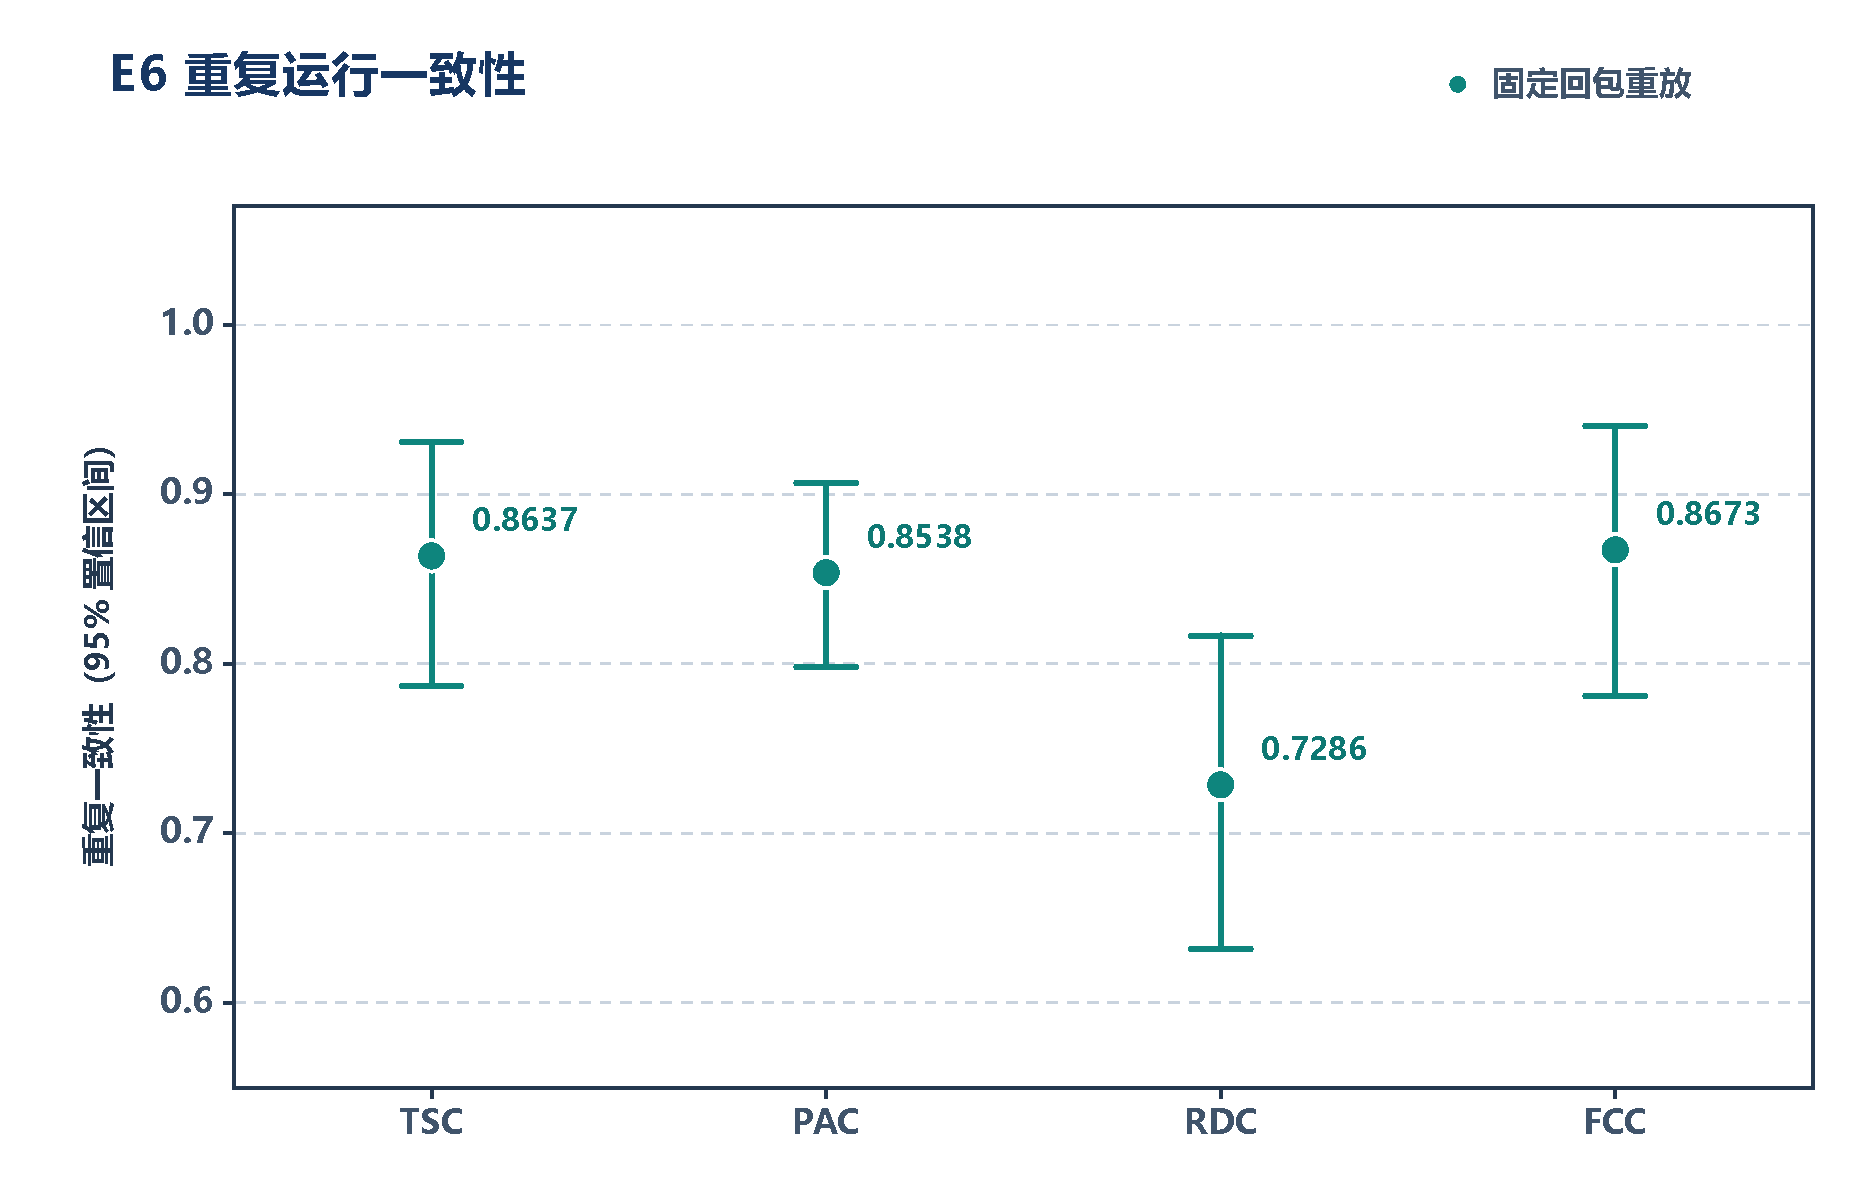
\includegraphics[width=\linewidth]{figures/fig6_e6.pdf}
\figcaption{重复运行一致性：TSC、PAC、RDC 与 FCC；误差线为按任务重抽样的 95\% 置信区间，估计基于 28 个具备至少两次有效重复的任务}{Repeated-run consistency (TSC, PAC, RDC and FCC) with task-bootstrap 95\% confidence intervals for 28 estimable tasks}
\label{fig:e6}
\end{columnfigure}

\begin{columntable}
\tabcaption{重复运行一致性与有效记录概况}{Summary of repeated-run consistency and valid records}
\label{tab:e6}
\fontsize{8bp}{10.5bp}\selectfont
\begin{tabularx}{\linewidth}{@{}>{\RaggedRight\arraybackslash}p{0.270\linewidth} >{\RaggedRight\arraybackslash}p{0.230\linewidth} >{\RaggedRight\arraybackslash}X@{}}
\toprule
\textbf{指标} & \textbf{结果} & \textbf{含义} \\
\midrule
有效记录率 & 133/160（83.13\%） & 满足有效记录条件的记录比例 \\
完整五次重复 & 21/32 个任务 & 具备完整重复序列的任务数 \\
可估计一致性 & 28/32 个任务 & 满足一致性估计条件的任务数 \\
TSC / PAC & 0.8637 / 0.8538 & 工具序列 / 参数设置一致性 \\
RDC / FCC & 0.7286 / 0.8673 & 返回数据 / 核心结论一致性 \\
\bottomrule
\end{tabularx}
\end{columntable}

\section{讨论}

本文将“模型是否理解并正确使用数据”与“程序是否按契约完成访问”拆开评价，再通过输入契约和统一结果结构考察两者的衔接。指导信息影响模型对字段、单位、缺失值和证据的使用；执行机制则对提交的操作和返回状态实施检查。这种分层使研究主张能够对应具体评价对象，避免将工具能够完成查询等同于科学解释正确。

E2 的固定场景与协议故障测试在字段与行集核对、成功零行与失败状态区分，以及分页和截断标记上给出核验结果。E4 的自然语言请求评价反映模型在语境中纠正、拒绝、澄清或停止的行为，不能以协议故障场景的通过率替代。程序对操作的约束为科学数据交付提供结构化依据，科学解释的质量仍需由 E3 单独评价。

E1 检验自然语言请求与工具及参数的对应关系，是模型是否理解并正确使用数据的直接证据：28 题三组回答的加权分均值为 0.9530，单位转换在三组均得满分，而澄清维度为 0.8333，说明确定查询条件之前的必要追问仍是主要改进方向。E1 与 E5 同属指导信息层的任务表现证据。

E5 的 B3 与 B2b 共享原子工具实现，比较结果显示，完整指导配置的规则通过率高 7.14 个百分点，工具调用和输出 token 分别减少 32.95\% 和 12.44\%。这些结果支持在该题集和生成预算下考察指导信息对模型决策、任务表现与运行开销的影响。指导消融保持程序执行约束一致，因此其差异不能作为相应程序模块独立贡献的估计。

A5 移除结果后验证指导后的通过率高于 B3。该比较评价模型指导，不涉及程序结果核验的独立作用。现有结果未显示该项指导能提高端到端通过率；其影响可结合失败轨迹中的额外操作、指令冲突和预算消耗进一步分析。

E3 中，完整配置相对于基础包装器在关键科学断言命中率、必要限定语覆盖率和严格合格率上表现更高。科学语义评分依据固定证据量规并采用模型辅助标注；结论对应 deepseek-v4.1-flash 模型及规定题集。

E6 分别量化工具序列、参数、数据和结论的跨次一致性，并通过有效记录比例说明可估计范围；其证据来自固定回包及有效记录条件。来源、状态和步骤记录为定位差异及数据复用提供了依据。

向其他天文档案迁移时，输入契约、状态分类、分页核验和结果来源关联可作为接口设计参考；字段语义、单位与缺失值约定、数据能力边界、认证方式及上游查询协议则须按数据源重新配置，并重新开展契约和科学语义评价。本文以 BEST 为实现与验证对象，所得结果为其他天文档案提供设计参考。

\section{结论与展望}

本文研究面向天文档案、具有科学语义约束的智能体数据访问方法，并以 BEST 为实现与验证对象。所提出的分层设计将面向模型决策的指导信息与面向查询操作的执行机制明确区分，通过输入契约和统一结果结构连接自然语言请求、查询执行与结果解释。访问工具和 TAP/ADQL 网关适配 BEST 两阶段查询，并关联查询条件、返回记录、状态与来源。

评价证据与两层设计分别对应：E2 的 21 个固定场景及 15 个协议故障场景均按约定处置；E5 在相同原子工具条件下，完整指导配置的规则通过率较基线高 7.14 个百分点，同时降低工具调用和输出 token 开销；E3 的关键科学断言命中率差值为 23.94 个百分点；E6 在固定回包与有效记录条件下的工具序列与核心结论一致性分别为 0.8637 和 0.8673。指导消融中的差异表明，增加指导信息不必然提升端到端表现，需要结合具体任务与操作轨迹分析。各组结论的适用范围见表~\ref{tab:claim-evidence} 与表~\ref{tab:strata}。

这些结果说明，科学档案智能体访问可以通过分别研究模型的数据理解和程序的契约执行，形成明确且可检验的研究主张。后续可针对不同档案重新配置领域语义与上游协议，在更多模型和任务中检验两层设计的衔接方式。

\section*{致谢}

待补充。

\section*{利益冲突声明}

作者声明本文不存在利益冲突。

\section*{AI 使用声明}

本文使用生成式人工智能辅助部分文字与图示的组织和润色。

\section*{数据与代码可用性}

访问工具、协议网关与评价代码公开于 \url{https://github.com/LL-LK/BEST}。

\begin{thebibliography}{99}
\RaggedRight

\bibitem{ref1} STOPPA F, BULMUS T, BLOEMEN S, et al. Textual interpretation of transient image classifications from large language models[J]. Nature Astronomy, 2025, 9(12): 1869-1878. DOI: 10.1038/s41550-025-02670-z.

\bibitem{ref2} WANG C, ZHANG Y, LI Y, et al. StarWhisper Telescope: an AI framework for automating end-to-end astronomical observations[J]. Communications Engineering, 2025, 4(1): 184. DOI: 10.1038/s44172-025-00520-4.

\bibitem{ref3} MANDAL I, SONI J, ZAKI M, et al. Evaluating large language model agents for automation of atomic force microscopy[J]. Nature Communications, 2025, 16(1): 9104. DOI: 10.1038/s41467-025-64105-7.

\bibitem{ref4} XIAO K. BEst STar (BEST) Database[DS/OL]. Version 1.0. Beijing: National Astronomical Observatories, Chinese Academy of Sciences, 2026-01-07 [2026-10-11]. \url{https://doi.org/10.12149/101651}

\bibitem{ref5} XIAO K, HUANG Y, YUAN H, et al. A Large and Precise All-Sky Photometric Standard Star Dataset Across More Than 200 Passbands[J]. Scientific Data, 2026, 13: 265. DOI: 10.1038/s41597-026-06590-z.

\bibitem{ref6} DOWLER P, RIXON G, TODY D, et al. Table Access Protocol, Version 1.1[S/OL]. International Virtual Observatory Alliance, 2019-09-27 [2026-10-11]. \url{https://www.ivoa.net/documents/TAP/}

\bibitem{ref13} DEMLEITNER M, DOWLER P, LUSTED J, et al. Astronomical Data Query Language, Version 2.1[S/OL]. International Virtual Observatory Alliance, 2023-12-15 [2026-10-22]. \url{https://www.ivoa.net/documents/ADQL/}

\bibitem{ref7} FAGHIH K, WANG W, CHENG Y, et al. Tool Preferences in Agentic LLMs are Unreliable[C]//Proceedings of the 2025 Conference on Empirical Methods in Natural Language Processing. Suzhou, China, 2025: 20954-20969. DOI: 10.18653/v1/2025.emnlp-main.1060.

\bibitem{ref8} GAIA COLLABORATION, VALLENARI A, et al. Gaia Data Release 3: Summary of the content and survey properties[J]. Astronomy \& Astrophysics, 2023, 674: A1. DOI: 10.1051/0004-6361/202243940.

\bibitem{ref9} GAIA DATA PROCESSING AND ANALYSIS CONSORTIUM. Gaia Data Release 3 Documentation, release 1.3[EB/OL]. European Space Agency, 2023-07-10 [2026-10-11]. \url{https://gea.esac.esa.int/archive/documentation/GDR3/}

\bibitem{ref10} YAO S, ZHAO J, YU D, et al. ReAct: Synergizing reasoning and acting in language models[C/OL]//International Conference on Learning Representations. Kigali, Rwanda, 2023 [2026-10-11]. \url{https://openreview.net/forum?id=WE_vluYUL-X}

\bibitem{ref11} CHEN Z, CHEN S, NING Y, et al. ScienceAgentBench: Toward rigorous assessment of language agents for data-driven scientific discovery[C/OL]//International Conference on Learning Representations. Singapore, 2025 [2026-10-11]. \url{https://proceedings.iclr.cc/paper_files/paper/2025/hash/f12b4df26344f3be803c06b555252efe-Abstract-Conference.html}

\bibitem{ref12} DING K, YU J, HUANG J, et al. SciToolAgent: A knowledge-graph-driven scientific agent for multitool integration[J]. Nature Computational Science, 2025, 5(10): 962-972. DOI: 10.1038/s43588-025-00849-y.

\bibitem{ref14} MCNEMAR Q. Note on the sampling error of the difference between correlated proportions or percentages[J]. Psychometrika, 1947, 12(2): 153-157. DOI: 10.1007/BF02295996.

\bibitem{ref15} FAGERLAND M W, LYDERSEN S, LAAKE P. The McNemar test for binary matched-pairs data: mid-p and asymptotic are better than exact conditional[J]. BMC Medical Research Methodology, 2013, 13: 91. DOI: 10.1186/1471-2288-13-91.

\end{thebibliography}

% 作者简介、照片及逐作者贡献说明按目标期刊要求另行提交。
\end{PaperBody}
\end{document}

